\section{AVL Trees}
If a binary tree is approximately \emph{balanced}, i.e.~if the left and right subtree of a binary tree $b$  have
roughly the same height, then the complexity of $b.\textsl{find}(k)$ will always be of the order
$\Oh\bigl(\ln(n)\bigr)$.  There are number of different variations of
balanced binary trees.  Of these variations, the species of balanced binary trees that is the easiest to understand is
called an \href{https://en.wikipedia.org/wiki/AVL_tree}{\emph{AVL tree}} \cite{adelson:62}.  AVl trees are 
named after their inventors \href{https://en.wikipedia.org/wiki/Georgy_Adelson-Velsky}{Georgy M.~Adelson-Velsky} 
and \href{https://en.wikipedia.org/wiki/Evgenii_Landis}{Evgenii~M.~Landis}.  In order to define these 
trees we need to define the \emph{height} of a binary tree formally:
\begin{enumerate}
\item $\textsl{Nil}.\textsl{height}() = 0$.
\item $\textsl{Node}(k,v,l,r).\textsl{height}() = 
       \max\bigl( l.\textsl{height}(), r.\textsl{height}() \bigr) + 1$. \eox
\end{enumerate}

\begin{Definition}[AVL-Tree] \hspace*{\fill} \\
{\em 
  The set $\AVL$ of \emph{AVL trees} is defined inductively:
  \begin{enumerate}
  \item $\textsl{Nil} \in \AVL$.
  \item $\textsl{Node}(k,v,l,r) \in \AVL$ \quad iff 
        \begin{enumerate}
        \item $\textsl{Node}(k,v,l,r) \in \Bin_<$,
        \item $l, r \in \AVL$ \quad and
        \item $|l.\textsl{height}() - r.\textsl{height}()| \leq 1$.

              This condition is called the \colorbox{orange}{\emph{balancing condition}}.
        \end{enumerate}
        According to this definition, an AVL tree is an ordered binary tree such that for every node
        $\textsl{Node}(k,v,l,r)$ in this tree the height of the left subtree $l$ and the right
        subtree  $r$ differ at most by 1.  \qed
  \end{enumerate}
}  
\end{Definition}

In order to implement AVL trees we can start from our implementation of ordered binary trees.
In addition to those methods that we have already seen in the class \textsl{Map} we will need the method
\\[0.2cm]
\hspace*{1.3cm} $\textsl{restore}: \Bin_< \rightarrow \AVL$. 
\\[0.2cm]
This method is used to restore the balancing condition at a given node if it has been violated by
either inserting or deleting an element.
The method call $b.\textsl{restore}()$ assumes that  $b$ is an ordered binary tree that satisfies
the balancing condition everywhere except possibly at its root. 
At the root, the height of the left subtree might differ from the height of the right subtree by at
most 2.  Hence, when the method $b.\textsl{restore}()$ is invoked we have either of the following
two cases:
\begin{enumerate}
\item $b = \textsl{Nil}$ \quad or
\item $b = \textsl{Node}(k,v,l,r) \wedge l \in \AVL \wedge r \in \AVL \wedge
       |l.\textsl{height}() - r.\textsl{height}()| \leq 2$.
\end{enumerate}
The method $\textsl{restore}$ is specified via conditional equations.
\begin{enumerate}
\item $\textsl{Nil}.\textsl{restore}() = \textsl{Nil}$,

      because the empty tree already is an  AVL tree.
\item $|l.\textsl{height}() - r.\textsl{height}()| \leq 1 \rightarrow 
       \textsl{Node}(k,v,l,r).\textsl{restore}() = \textsl{Node}(k,v,l,r)$,

      because if the balancing condition is already satisfied, then nothing needs to be done. 
\item $\begin{array}[t]{cl}
              & l_1.\textsl{height}() = r_1.\textsl{height}() + 2    \\ 
       \wedge & l_1 = \textsl{Node}(k_2,v_2,l_2,r_2)                 \\
       \wedge & l_2.\textsl{height}() \geq r_2.\textsl{height}()     \\[0.2cm]
       \rightarrow & \textsl{Node}(k_1,v_1,l_1,r_1).\textsl{restore}() = 
                     \textsl{Node}\bigl(k_2,v_2,l_2,\textsl{Node}(k_1,v_1,r_2,r_1)\bigr)
       \end{array}
      $

      The motivation for this equation can be found in Figure \ref{fig:casell}
      on page \pageref{fig:casell}.  The left part of this figure shows the state
      of the tree before it has been rebalanced.  Therefore, this part shows the tree
      \\[0.2cm]
      \hspace*{1.3cm}
      $\textsl{Node}(k_1,v_1, \textsl{Node}(k_2,v_2,l_2,r_2), r_1)$. 
      \\[0.2cm]
      The right part of Figure \ref{fig:casell} shows the effect of rebalancing.  
      This rebalancing results in the tree
      \\[0.2cm]
      \hspace*{1.3cm}
      $\textsl{Node}\bigl(k_2,v_2,l_2,\textsl{Node}(k_1,v_1,r_2,r_1)\bigr)$.
      \\[0.2cm]
      In Figure \ref{fig:casell} the label below the horizontal line of each node shows the height
      of the tree corresponding to this node.  For subtrees, the height is given below the name of
      the subtree.  For example,  $h$ is the height of the subtree 
      $l_2$, while $h-1$ is the height of the subtree $r_1$. The height of the subtree $r_2$
      is $h'$ and we know that $h' \leq h$.  As $\textsl{Node}(k_2,v_2,l_2,r_2)$ is an AVL tree and we know that
      $l_2.\textsl{height}() \geq r_2.\textsl{height}()$, we
      either have $h' = h$ or $h' = h-1$.

      The state shown in Figure \ref{fig:casell} can arise if either an element has been inserted
      in the left subtree $l_1$ or if an element has been deleted from the right subtree  $r_1$.

      \begin{figure}[!ht]
        \centering
        \framebox{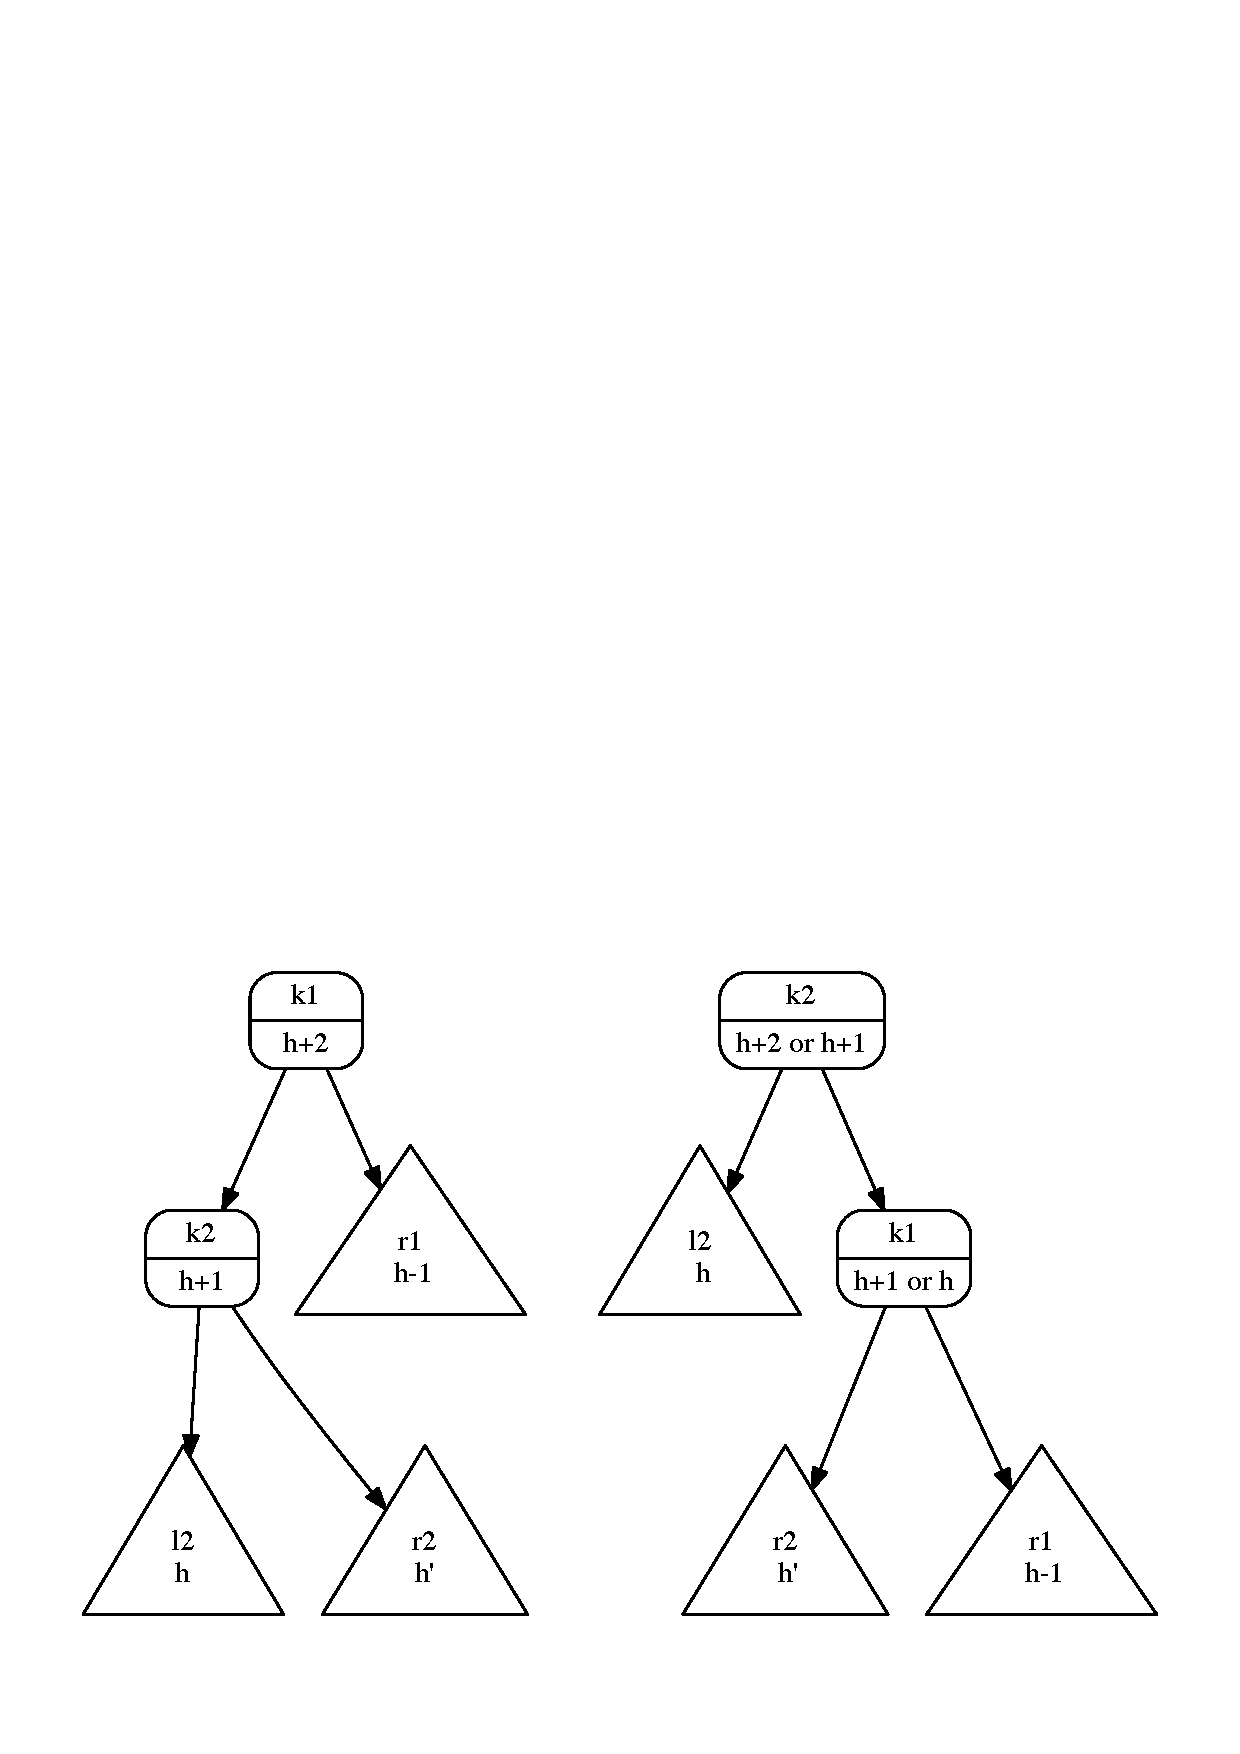
\epsfig{file=Abbildungen/casell,scale=0.7}} 
        \caption{An unbalanced tree and the corresponding rebalanced tree.}
        \label{fig:casell}
      \end{figure}
      We have to make sure that the tree shown in the right part of Figure
      \ref{fig:casell} is indeed an  AVL tree. With respect to the balancing condition this is
      easily verified.  The fact that the node containing the key $k_1$ has either the height
      $h$ or $h+1$ is a consequence of the fact that the height of $r_1$ is  $h-1$ and that  $h' \in \{h, h-1\}$.

      In order to verify that the tree is ordered we can use the following inequation: 
      \\[0.2cm]
      \hspace*{1.3cm}
      $l_2 < k_2 < r_2 < k_1 < r_1$. 
      \hspace*{\fill} $(\star)$
      \\[0.2cm]
      Here we have used the following notation: If  $k$ is a key and  $b$ is a binary tree, then we write \\[0.2cm]
      \hspace*{1.3cm} $k < b$ \\[0.2cm]
      in order to express that  $k$ is smaller than all keys that occur in the tree  $b$.
      Similarly,  $b < k$ denotes the fact that all keys occuring in $b$ are less than the key
      $k$.  The inequation  $(\star)$ describes both the ordering of keys in the left part of Figure
      \ref{fig:casell} and in the right part of this figure.  Hence, the tree shown in the right
      part of Figure \ref{fig:casell} is ordered provided the tree in the left part is ordered to begin with.
\item $\begin{array}[t]{cl}
               & l_1.\textsl{height}() = r_1.\textsl{height}() + 2    \\ 
        \wedge & l_1 = \textsl{Node}(k_2,v_2,l_2,r_2)               \\
        \wedge & l_2.\textsl{height}() < r_2.\textsl{height}()     \\
        \wedge & r_2 = \textsl{Node}(k_3,v_3,l_3,r_3)               \\
        \rightarrow & \textsl{Node}(k_1,v_1,l_1,r_1).\textsl{restore}() = 
                      \textsl{Node}\bigl(k_3,v_3,\textsl{Node}(k_2,v_2,l_2,l_3),\textsl{Node}(k_1,v_1,r_3,r_1) \bigr)
        \end{array}
       $

       The left hand side of this equation is shown in Figure  \ref{fig:caselr} on page
       \pageref{fig:caselr}.  This tree can be written as
       \\[0.2cm]
       \hspace*{1.3cm} 
       $\textsl{Node}\bigl(k_1,v_1,\textsl{Node}(k_2,v_2,l_2,\textsl{Node}\bigl(k_3,v_3,l_3,r_3)\bigr),r_1\bigr)$. 
       \\[0.2cm]
       The subtrees $l_3$ and $r_3$ have either the height  $h$ or $h-1$.  Furthermore, at least one
       of these subtrees must have the height  $h$ for otherwise the subtree
       $\textsl{Node}(k_3,v_3,l_3,r_3)$ would not have the height $h+1$.
       
\begin{figure}[!ht]
  \centering
  \framebox{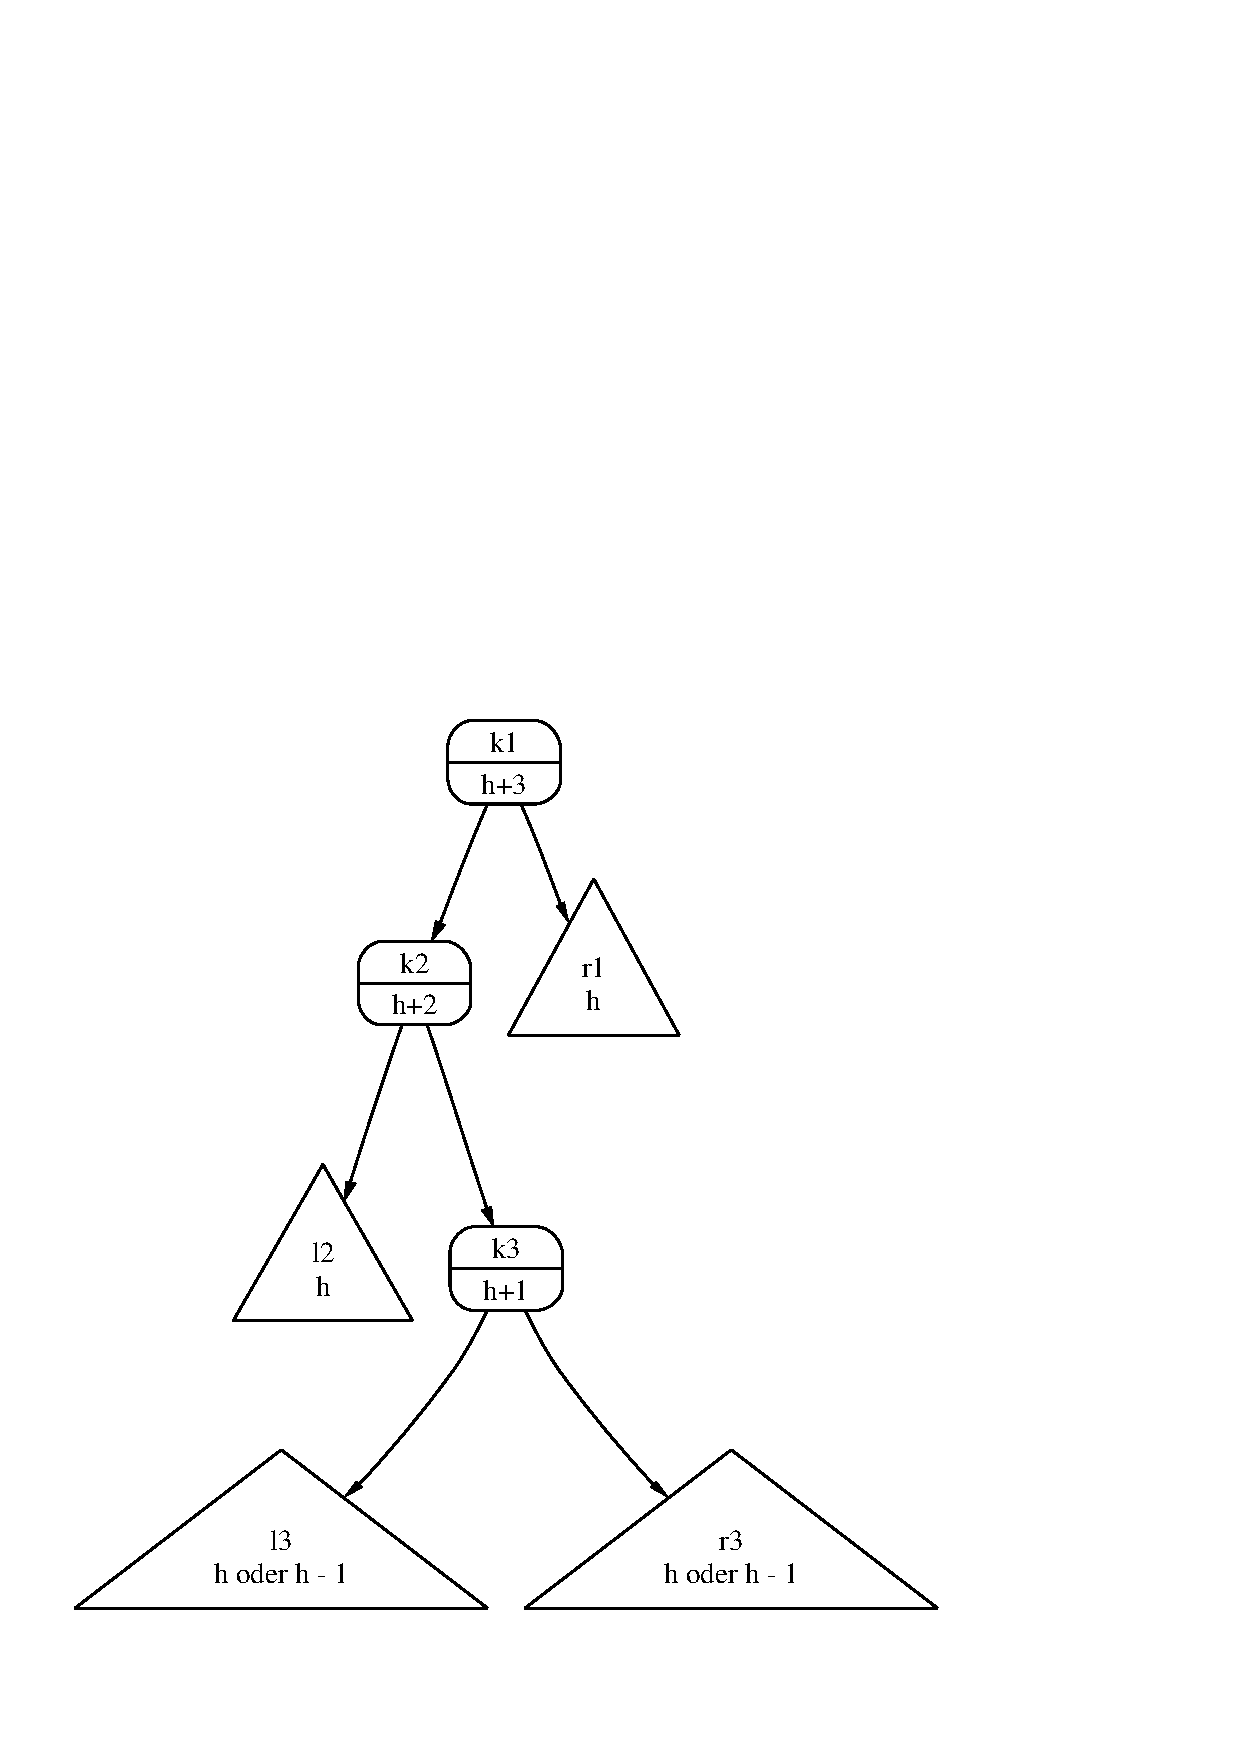
\epsfig{file=Abbildungen/caselr,scale=0.7}} 
  \caption{An unbalanced tree, second case.}
  \label{fig:caselr}
\end{figure}

     Figure \ref{fig:caselr-nach} on page \pageref{fig:caselr-nach} shows how the tree looks after
     rebalancing.  The tree shown in this figure has the form
     \\[0.2cm]
     \hspace*{1.3cm} 
     $\textsl{Node}\bigl(k_3,v_3,\textsl{Node}(k_2,v_2,l_2,l_3),\textsl{Node}(k_1,v_1,r_3,r_1) \bigr)$.


\begin{figure}[!ht]
  \centering
  \framebox{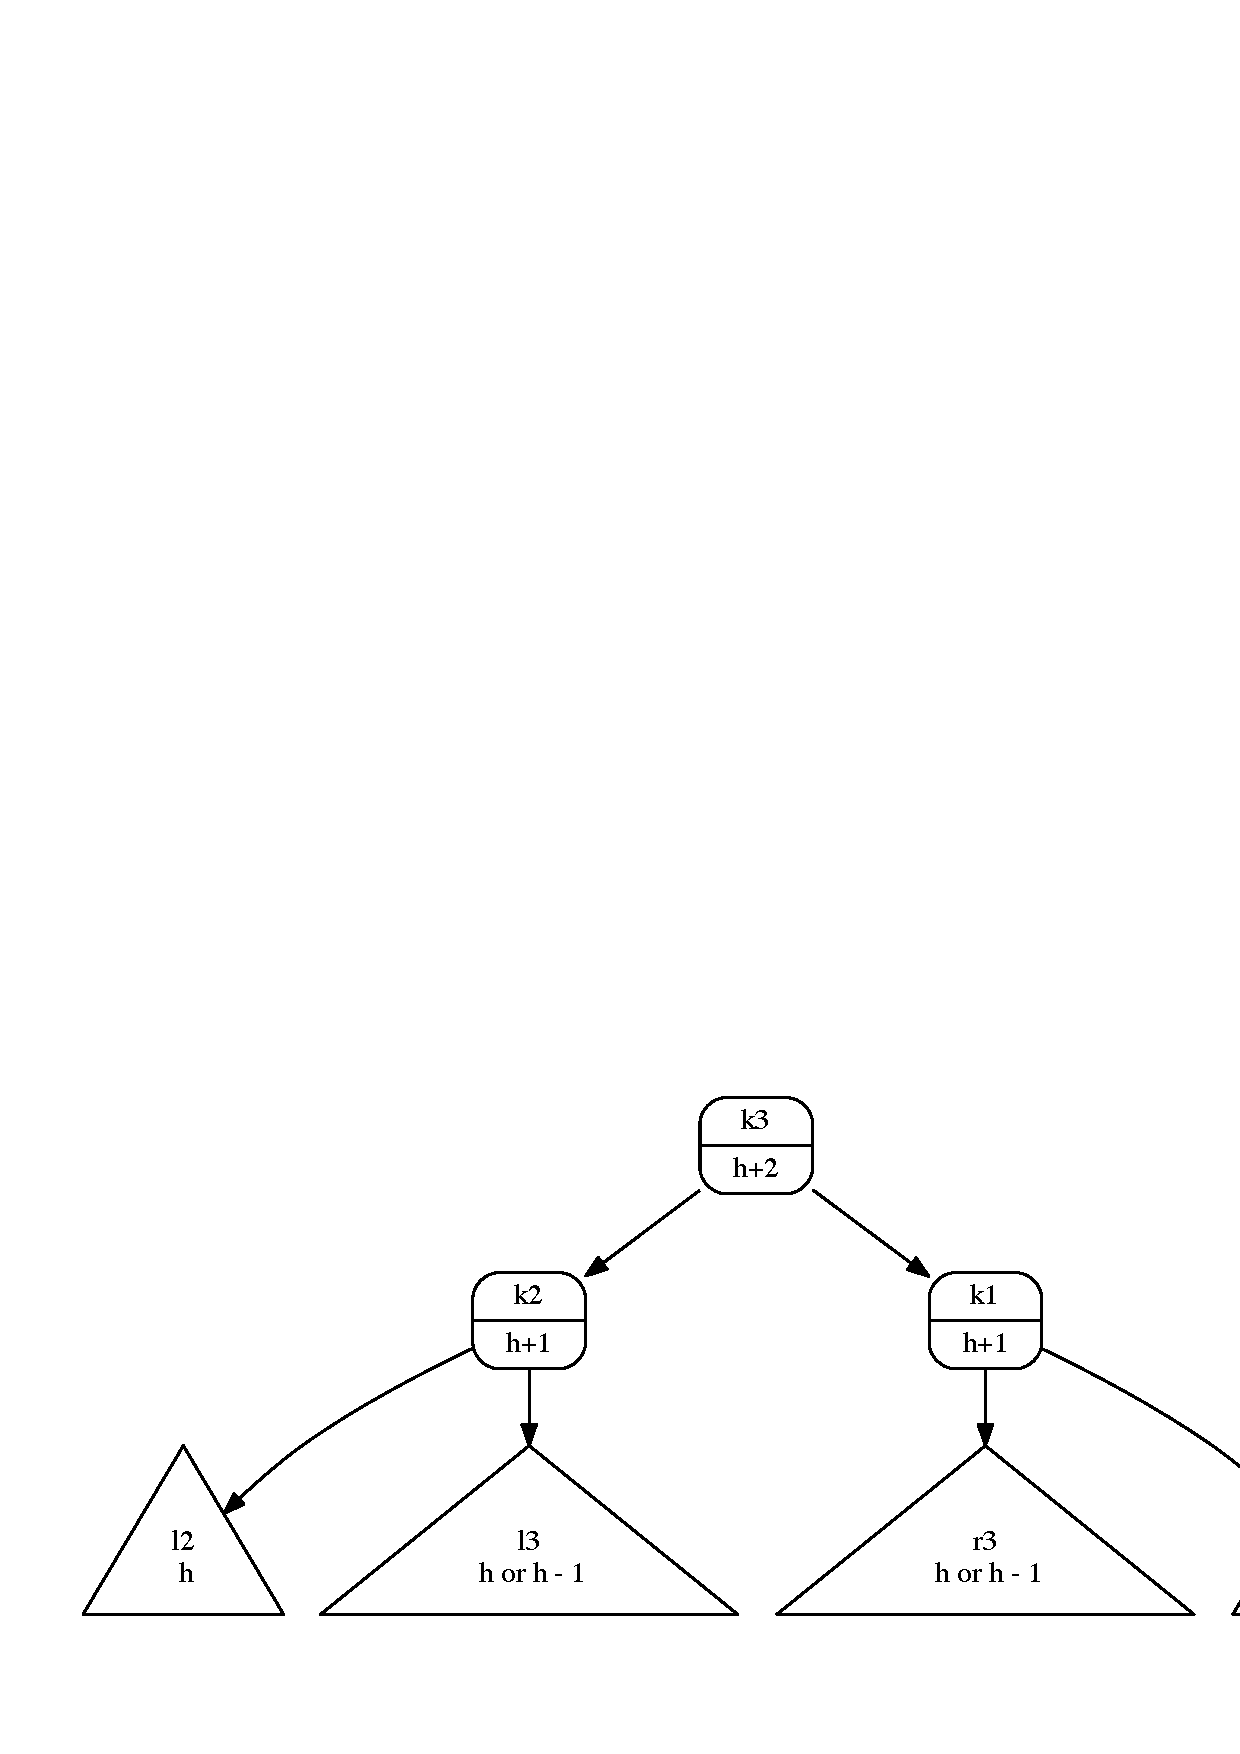
\epsfig{file=Abbildungen/caselr-nach,scale=0.7}} 
  \caption{The rebalanced tree in the second case.}
  \label{fig:caselr-nach}
\end{figure}

      The inequation describing the ordering of the keys both in the left subtree and in the right
      subtree is given as
      \\[0.2cm]
      \hspace*{1.3cm} $l_2 < k_2 < l_3 < k_3 < r_3 < k_1 < r_1$.

      There are two more cases where the height of the right subtree is bigger by more than 
      the height of the left subtree plus one.  These two cases are completely analogous to the two
      cases discussed previously.  Therefore we just state the corresponding equations without
      further discussion.
\item $\begin{array}[t]{cl}
              & r_1.\textsl{height}() = l_1.\textsl{height}() + 2    \\ 
       \wedge & r_1 = \textsl{Node}(k_2,v_2,l_2,r_2)               \\
       \wedge & r_2.\textsl{height}() \geq l_2.\textsl{height}()     \\[0.2cm]
       \rightarrow & \textsl{Node}(k_1,v_1,l_1,r_1).\textsl{restore}() = 
                     \textsl{Node}\bigl(k_2,v_2,\textsl{Node}(k_1,v_1,l_1,l_2),r_2\bigr)
       \end{array}
      $
\item $\begin{array}[t]{cl}
               & r_1.\textsl{height}() = l_1.\textsl{height}() + 2    \\ 
        \wedge & r_1 = \textsl{Node}(k_2,v_2,l_2,r_2)               \\
        \wedge & r_2.\textsl{height}() < l_2.\textsl{height}()     \\
        \wedge & l_2 = \textsl{Node}(k_3,v_3,l_3,r_3)               \\
        \rightarrow & \textsl{Node}(k_1,v_1,l_1,r_1).\textsl{restore}() = 
                      \textsl{Node}\bigl(k_3,v_3,\textsl{Node}(k_1,v_1,l_1,l_3),\textsl{Node}(k_2,v_2,r_3,r_2) \bigr)
        \end{array}
       $

\end{enumerate}
Now we are ready to specify the method  $\textsl{insert}()$ via recursive equations.
If we compare these equations to the equations we had given for unbalanced ordered binary trees we
notice that we only have to call the method $\textsl{restore}$ if the balancing condition might have
been violated.
\begin{enumerate}
\item $\textsl{Nil}.\textsl{insert}(k,v) = \textsl{Node}(k,v, \textsl{Nil}, \textsl{Nil})$.  
\item $\textsl{Node}(k, v_2, l, r).\textsl{insert}(k,v_1) = \textsl{Node}(k, v_1, l, r)$.
\item $k_1 < k_2 \rightarrow 
          \textsl{Node}(k_2, v_2, l, r).\textsl{insert}(k_1, v_1) =
          \textsl{Node}\bigl(k_2, v_2, l.\textsl{insert}(k_1,v_1), r\bigr).\textsl{restore}()$.
\item $k_1 > k_2 \rightarrow 
         \textsl{Node}(k_2, v_2, l, r).\textsl{insert}\bigl(k_1, v_1\bigr) = 
         \textsl{Node}\bigl(k_2, v_2, l, r.\textsl{insert}(k_1,v_1)\bigr).\textsl{restore}()$.
\end{enumerate}
The equations for  $\textsl{delMin}()$ change as follows:
\begin{enumerate}
\item $\textsl{Node}(k, v, \textsl{Nil}, r).\textsl{delMin}() = \langle r, k, v \rangle$.
\item $l\not= \textsl{Nil} \wedge \langle l',k_{min}, v_{min}\rangle := l.\textsl{delMin}() 
       \;\rightarrow$ \\[0.2cm]
       \hspace*{1.3cm} 
       $\textsl{Node}(k, v, l, r).\textsl{delMin}() = 
        \langle \textsl{Node}(k, v, l', r).\textsl{restore}(), k_{min}, v_{min} \rangle$.
\end{enumerate}
Then, the equations for \textsl{delete} are as follows:
\begin{enumerate}
\item $\textsl{Nil}.\textsl{delete}(k) = \textsl{Nil}$.
\item $\textsl{Node}(k,v,\textsl{Nil},r).\textsl{delete}(k) = r$.
\item $\textsl{Node}(k,v,l,\textsl{Nil}).\textsl{delete}(k) = l$.
\item $l \not= \textsl{Nil} \,\wedge\, r \not= \textsl{Nil} \,\wedge\, 
       \langle r',k_{min}, v_{min} \rangle := r.\textsl{delMin}()  \;\rightarrow$ \\[0.2cm]
      \hspace*{1.3cm}
      $\textsl{Node}(k,v,l,r).\textsl{delete}(k) = \textsl{Node}(k_{min},v_{min},l,r').\textsl{restore}()$.
\item $k_1 < k_2 \rightarrow \textsl{Node}(k_2,v_2,l,r).\textsl{delete}(k_1) = 
       \textsl{Node}\bigl(k_2,v_2,l.\textsl{delete}(k_1),r\bigr).\textsl{restore}()$.
\item $k_1 > k_2 \rightarrow \textsl{Node}(k_2,v_2,l,r).\textsl{delete}(k_1) = 
         \textsl{Node}\bigl(k_2,v_2,l,r.\textsl{delete}(k_1)\bigr).\textsl{restore}()$.
\end{enumerate}


\subsection{Implementing AVL-Trees in \textsc{SetlX}}
If we want to implement AVL-trees in \textsc{SetlX} then we have to decide how to compute the height
of the trees.  The idea is to store the height of every subtree in the corresponding node since it
would be inefficient if we would recompute this height every time we need it.  Therefore, we add a
member variable \texttt{mHeight} to our class map.
Figure \ref{fig:avl-tree.stlx:outline} shows an outline of the class \texttt{map}.  The variable
\texttt{mHeight} is defined in line 6.  It is initialised as $0$ since the constructor \texttt{map}
constructs an empty node.  

\begin{figure}[!ht]
  \centering
\begin{Verbatim}[ frame         = lines, 
                  framesep      = 0.3cm, 
                  labelposition = bottomline,
                  numbers       = left,
                  numbersep     = -0.2cm,
                  xleftmargin   = 0.0cm,
                  xrightmargin  = 0.0cm
                ]
    class map(cmp) {
        mKey    := om;
        mValue  := om; 
        mLeft   := om;
        mRight  := om;
        mHeight := 0;
        mCmpFct := cmp;  
    
      static {
        isEmpty       := [] |-> mKey == om;
        find          := procedure(k)          { ... };
        insert        := procedure(k, v)       { ... };
        delMin        := procedure()           { ... };
        delete        := procedure(k)          { ... };
        update        := procedure(t)          { ... };
        restore       := procedure()           { ... };
        setValues     := procedure(k, v, l, r) { ... };
        restoreHeight := procedure()           { ... };
      }
    }
\end{Verbatim}
\vspace*{-0.3cm}
  \caption{Outline of the class \texttt{map}.}
  \label{fig:avl-tree.stlx:outline}
\end{figure}


Figure \ref{fig:avl-tree.stlx:find} show the implementation of the function \texttt{find}.
Actually, the implementation is the same as the implementation in Figure
\ref{fig:binary-tree.stlx-1}.  The reason is that every AVL tree is also an ordered binary tree and
since searching for a key does not change the underlying tree there is no need to restore anything.

\begin{figure}[!ht]
\centering
\begin{Verbatim}[ frame         = lines, 
                  framesep      = 0.3cm, 
                  firstnumber   = 1,
                  labelposition = bottomline,
                  numbers       = left,
                  numbersep     = -0.2cm,
                  xleftmargin   = 0.8cm,
                  xrightmargin  = 0.8cm,
                ]
    find := procedure(k) {
        if      (isEmpty())        { return;                }
        else if (mKey == k)        { return mValue;         }
        else if (mCmpFct(k, mKey)) { return mLeft .find(k); }
        else                       { return mRight.find(k); }
    };
\end{Verbatim}
\vspace*{-0.3cm}
\caption{Implementation of the method \texttt{find}.}
\label{fig:avl-tree.stlx:find}
\end{figure}


Figure \ref{fig:avl-tree.stlx:insert} shows the implementation of the method \texttt{insert}.
If we compare this implementation with the implementation for binary trees, we find three
differences.
\begin{enumerate}
\item When inserting into an empty tree, we now have to update the member variable \texttt{mHeight}
      to $1$.  This is done in line 7.
\item After inserting a value into the left subtree \texttt{mLeft}, it might be necessary to 
      rebalance the tree.  This is done in line 12.
\item Similarly, if we insert a value into the right subtree \texttt{mRight}, we have to rebalance 
      the tree.  This is done in line 15.
\end{enumerate}

\begin{figure}[!ht]
\centering
\begin{Verbatim}[ frame         = lines, 
                  framesep      = 0.3cm, 
                  firstnumber   = 1,
                  labelposition = bottomline,
                  numbers       = left,
                  numbersep     = -0.2cm,
                  xleftmargin   = 0.8cm,
                  xrightmargin  = 0.8cm,
                ]
    insert := procedure(k, v) {
        if (isEmpty()) { 
            this.mKey    := k;
            this.mValue  := v; 
            this.mLeft   := map(mCmpFct);
            this.mRight  := map(mCmpFct);
            this.mHeight := 1;
        } else if (mKey == k) { 
            this.mValue := v; 
        } else if (mCmpFct(k, mKey)) { 
            mLeft.insert(k, v); 
            restore();
        } else { 
            mRight.insert(k, v); 
            restore();
        }
    };
\end{Verbatim}
\vspace*{-0.3cm}
\caption{Implementation of the method \texttt{insert}.}
\label{fig:avl-tree.stlx:insert}
\end{figure}

Figure \ref{fig:avl-tree.stlx:delMin} shows the implementation of the method \texttt{delMin}.
The only change compared to the previous implementation for ordered binary trees is in line 7, where
we have to take care of the fact that the balancing condition might be violated after deleting the
smallest element in the left subtree.

\begin{figure}[!ht]
\centering
\begin{Verbatim}[ frame         = lines, 
                  framesep      = 0.3cm, 
                  firstnumber   = 1,
                  labelposition = bottomline,
                  numbers       = left,
                  numbersep     = -0.2cm,
                  xleftmargin   = 0.8cm,
                  xrightmargin  = 0.8cm,
                ]
    delMin := procedure() {
        if (mLeft.isEmpty()) { 
            return [ mRight, mKey, mValue ]; 
        } else {
             [ ls, km, vm ] := mLeft.delMin();
             this.mLeft := ls;
             restore();
             return [ this, km, vm ];
        }
    };
\end{Verbatim}
\vspace*{-0.3cm}
\caption{Implementation of \texttt{delMin}.}
\label{fig:avl-tree.stlx:delMin}
\end{figure}

\pagebreak
Figure \ref{fig:avl-tree.stlx:delete} shows the implementation of the method \texttt{delete} and the
implementation of the auxiliary method \texttt{update}.  Compared with Figure
\ref{fig:binary-tree.stlx-2} there are only three differences:
\begin{enumerate}
\item If we delete the key at the root of the tree, we replace this key with the smallest key in the
      right subtree.  Since this key is deleted in the right subtree, the height of the right
      subtree might shrunk and hence the balancing condition at the root might be violated.
      Therefore, we have to restore the balancing condition.  This is done in line 12.
\item If we delete a key in the left subtree, the height of the left subtree might shrink.
      Hence we have to rebalance the tree at the root in line 16.
\item Similarly, if we delete a key in the right subtree, we have to restore the balancing
      condition.  This is done in line 19.
\end{enumerate}
Of course, since the method \texttt{update} only sets the member variables of the tree, it does not
change the structure of the tree.  Hence there is no need for a call to \texttt{restore} in this method.

\begin{figure}[!ht]
\centering
\begin{Verbatim}[ frame         = lines, 
                  framesep      = 0.3cm, 
                  firstnumber   = 1,
                  labelposition = bottomline,
                  numbers       = left,
                  numbersep     = -0.2cm,
                  xleftmargin   = 0.0cm,
                  xrightmargin  = 0.0cm,
                ]
    delete := procedure(k) {
        if (isEmpty())  { 
            return; 
        } else if (k == mKey) {
            if (mLeft.isEmpty()) {
                update(mRight);
            } else if (mRight.isEmpty()) {
                update(mLeft);
            } else {
                [ rs, km, vm ] := mRight.delMin();
                [this.mKey,this.mValue,this.mRight ] := [km,vm,rs];
                restore();
            }
        } else if (mCmpFct(k, mKey)) {
            mLeft.delete(k);
            restore();
        } else {
            mRight.delete(k);
            restore();
        }
    };
    update := procedure(t) {
        this.mKey    := t.mKey;
        this.mValue  := t.mValue;
        this.mLeft   := t.mLeft;
        this.mRight  := t.mRight;
        this.mHeight := t.mHeight;
    };
\end{Verbatim}
\vspace*{-0.3cm}
\caption{The methods \texttt{delete} and \texttt{update}.}
\label{fig:avl-tree.stlx:delete}
\end{figure}
\begin{figure}[!ht]
\centering
\begin{Verbatim}[ frame         = lines, 
                  framesep      = 0.3cm, 
                  firstnumber   = 1,
                  labelposition = bottomline,
                  numbers       = left,
                  numbersep     = -0.2cm,
                  xleftmargin   = 0.0cm,
                  xrightmargin  = 0.0cm,
                ]
    restore := procedure() {
        if (abs(mLeft.mHeight - mRight.mHeight) <= 1) {
            restoreHeight();
            return;
        }
        if (mLeft.mHeight > mRight.mHeight) {
            [ k1,v1,l1,r1 ] := [ mKey,mValue,mLeft,mRight ];
            [ k2,v2,l2,r2 ] := [ l1.mKey,l1.mValue,l1.mLeft,l1.mRight ];
            if (l2.mHeight >= r2.mHeight) {
                setValues(k2,v2,l2,createNode(k1,v1,r2,r1,mCmpFct));
            } else {
                [ k3,v3,l3,r3 ] := [r2.mKey,r2.mValue,r2.mLeft,r2.mRight];
                setValues(k3,v3,createNode(k2,v2,l2,l3,mCmpFct),
                                createNode(k1,v1,r3,r1,mCmpFct) );
            }
        }
        if (mRight.mHeight > mLeft.mHeight) {
            [ k1,v1,l1,r1 ] := [ mKey,mValue,mLeft,mRight ];
            [ k2,v2,l2,r2 ] := [ r1.mKey,r1.mValue,r1.mLeft,r1.mRight ];
            if (r2.mHeight >= l2.mHeight) {
                setValues(k2,v2,createNode(k1,v1,l1,l2,mCmpFct),r2);
            } else {
                [ k3,v3,l3,r3 ] := [l2.mKey,l2.mValue,l2.mLeft,l2.mRight];
                setValues(k3,v3,createNode(k1,v1,l1,l3,mCmpFct),
                                createNode(k2,v2,r3,r2,mCmpFct) );
            }
        }
        restoreHeight();
    };
    setValues := procedure(k, v, l, r) {
        this.mKey   := k;
        this.mValue := v;
        this.mLeft  := l;
        this.mRight := r;
    };
    restoreHeight := procedure() {
        this.mHeight := 1 + max({ mLeft.mHeight, mRight.mHeight });
    };
\end{Verbatim}
\vspace*{-0.3cm}
\caption{The implementation of \texttt{restore} and \texttt{restoreHeight}.}
\label{fig:avl-tree.stlx:restore}
\end{figure}


Figure \ref{fig:avl-tree.stlx:restore} shows the implementation of the function \texttt{restore}.
It is this method that makes most of the difference between ordered binary trees and AVL trees.  Let
us discuss this method line by line.
\begin{enumerate}
\item In line 2 we check whether the balancing condition is satisfied.  If we are lucky,  this test 
      is successful and hence we do not need to restore the structure of the tree.  However, we
      still need to maintain the height of the tree since it is possible that variable
      \texttt{mHeight} no longer contains the correct height.  For example, assume that the left subtree
      initially has a height that is bigger by one than the height of the right subtree.  Assume
      further that we have deleted a node in the left subtree so that its height shrinks.  Then the
      balancing condition is still satisfied, as now the left subtree and the right subtree have the
      same height.  However, the height of the complete tree has also shrunk by one and therefore, 
      the variable \texttt{mHeight} needs to be decremented.  This is done via the auxiliary method
      \texttt{restoreHeight}.  This method is defined in line 36 and it recomputes \texttt{mHeight}
      according to the definition of the height of a binary tree.
\item If the check in line 2 fails, then we know that the balancing condition is violated.
      However, we do not yet know which of the two subtrees is bigger.  

      If the test in line 6 succeeds, then the left subtree must have a height that is bigger by
      two than the height of the right subtree.  In order to be able to use the same variable names 
      as the variable names given in the equations discussed in the previous subsection, we define
      the variables \texttt{k1}, \texttt{v1}, $\cdots$, \texttt{l2}, and \texttt{r2} in line 7 and 8
      so that these variable names correspond exactly to the variable names used in the Figures
      \ref{fig:casell} and \ref{fig:caselr}.
\item Next, the test in line 9 checks whether we have the case that is depicted in Figure
      \ref{fig:casell}.  In this case, Figure \ref{fig:casell} tells us that the key \texttt{k2}
      has to move to the root.  The left subtree is now \texttt{l2}, while the right subtree is a
      new node that has the key \texttt{k1} at its root.  This new node is created by the call
      of the function \texttt{createNode} in line 10.  The function \texttt{createNode} is shown in
      Figure \ref{fig:avl-tree.stlx:createNode} on page \pageref{fig:avl-tree.stlx:createNode}.
\item If the test in line 9 fails, the right subtree is bigger than the left subtree and we are in 
      the case that is depicted in Figure \ref{fig:caselr}.  We have to create the tree that is
      shown in Figure \ref{fig:caselr-nach}.  To this end we first define the variables 
      \texttt{k3}, \texttt{v3}, \texttt{l3}, and \texttt{r3} in a way that these variables
      correspond to the variables shown in Figure \ref{fig:caselr}.  Next, we create the tree
      that is shown in Figure \ref{fig:caselr-nach}.
\item Line 17 deals with the case that the right subtree is bigger than the left subtree. 
      As this case is analogous to the case covered in line 6 to line 16, we won't discuss this case
      any further.
\item Finally, we recompute the variable \texttt{mHeight} since it is possible that the old value is
      no longer correct.
\end{enumerate}


\begin{figure}[!ht]
\centering
\begin{Verbatim}[ frame         = lines, 
                  framesep      = 0.3cm, 
                  firstnumber   = 1,
                  labelposition = bottomline,
                  numbers       = left,
                  numbersep     = -0.2cm,
                  xleftmargin   = 0.8cm,
                  xrightmargin  = 0.8cm,
                ]
    createNode :=  procedure(key, value, left, right, cmp) {
        node         := map(cmp);
        node.mKey    := key;
        node.mValue  := value;
        node.mLeft   := left;
        node.mRight  := right;
        node.mCmpFct := cmp;
        node.mHeight := 1 + max({ left.mHeight, right.mHeight });
        return node;
    };
\end{Verbatim}
\vspace*{-0.3cm}
\caption{}
\label{fig:avl-tree.stlx:createNode}
\end{figure}

The function \texttt{createNode} shown in Figure \ref{fig:avl-tree.stlx:createNode}
constructs a node with given left and right subtrees.  In fact, this method serves as a second
constructor for the class \texttt{map}.  The implementation should be obvious.


\subsection{Analysis of the Complexity of AVL Trees}
Next, we analyze the complexity of AVL trees in the worst case.  In order to do this we have to know
what the worst case actually looks like.  Back when we only had ordered binary trees the worst case was the case where
the tree had degenerated into a list.  Now, the worst case is the case where the tree is as slim as
it can possibly be while still satisfying the definition of an AVL tree.  Hence the worst case
happens if the tree has a given height $h$ but the number of keys stored in the tree is as small as
possible.  To investigate trees of this kind, let us define  $b_h(k)$ as an AVL tree that has height
$h$ and whose number of keys is minimal among all other AVL trees of given  height $h$.  Furthermore,
we demand that all keys stored in  $b_h(k)$ are bigger than  $k$.  For our investigation of the
complexity, both the keys and the values do not really matter.  The only problem is that we have to
make sure that the tree $b_h(k)$ that we are going to construct in a moment is actually an ordered
tree and for this reason we insist that all keys in $b_h(k)$ are bigger than $k$.  We will use
natural numbers as keys, while all values will be $0$.
Before we can actually present the definition of  $b_h(k)$ we need to define the auxiliary function
 $\textsl{maxKey}()$.  This function has the signature 
\\[0.2cm]
\hspace*{1.3cm}
$\textsl{maxKey}:\mathcal{B}_< \rightarrow \textsl{Key} \cup \{ \Omega \}$.
\\[0.2cm]
Given a non-empty ordered binary tree  $b$, the expression $b.\textsl{maxKey}()$ returns the biggest
key stored in $b$.  The expression  $b.\textsl{maxKey}()$ is defined by induction on $b$:
\begin{enumerate}
\item $\textsl{Nil}.\textsl{maxKey}() = \Omega$,
\item $\textsl{Node}(k,v,l,\textsl{Nil}).\textsl{maxKey}() = k$,
\item $r \not= \textsl{Nil} \rightarrow \textsl{Node}(k,v,l,r).\textsl{maxKey}() = r.\textsl{maxKey}()$.
\end{enumerate}
Now we are ready to define the trees  $b_h(k)$ by induction on  $h$.
\begin{enumerate}
\item $b_0(k) = \textsl{Nil}$,

      because there is only one AVL tree of height $0$ and this is the tree \textsl{Nil}.
\item $b_1(k) = \textsl{Node}(k+1,0,\textsl{Nil}, \textsl{Nil})$,

      since, if we abstract from the actual keys and values, there is exactly one AVL tree of height
      $1$.
\item $b_{h+1}(k).\textsl{maxKey}() = l \rightarrow 
       b_{h+2}(k) = \textsl{Node}\bigl(l+1,\,0,\,b_{h+1}(k),\,b_h(l+1)\bigr)$.

      In order to construct an AVL tree of height $h+2$ that contains the minimal number of keys 
      possible we first construct the AVL tree $b_{h+1}(k)$ which has height  $h+1$ and which stores as few
      key as possible given its height.  Next, we determine the biggest key $l$ in this tree. 
      Now to construct $b_{h+2}(k)$ we take a node with the key $l+1$ as the root.
      The left subtree of this node is $b_{h+1}(k)$, while the right subtree is $b_h(l+1)$.
      Since $l$ is the biggest key in $b_{h+1}(k)$, all key in the left subtree of
      $b_{h+2}(k)$ are indeed smaller than the key $l+1$ at the root.  Since all keys in
      $b_h(l+1)$ are bigger than $l+1$, the keys in the right subtree are bigger than the key at the
      root.  Therefore, $b_{h+2}(k)$ is an ordered binary tree.

      Furthermore, $b_{h+2}(k)$ is an AVL tree of height $h+2$ since the height of the left subtree
      is $h+1$ and the height of the right subtree is $h$.  Also, this tree is as slim as
      any AVL tree can possibly get, since if the left subtree has height $h+1$ the right subtree
      must at least have height $h$ in order for the whole tree to be an AVL tree.
\end{enumerate}
Let us denote the number of keys stored in a binary tree $b$ as  $\#\,b$.  Furthermore, we define
\\[0.2cm]
\hspace*{1.3cm}
$c_h := \#\, b_h(k)$
\\[0.2cm]
to be the number of keys in the tree $b_h(k)$.  We will see immediately that 
$\#\,b_h(k)$ does not depend on the number $k$ and therefore $c_h$ does not depend on $k$.  Starting
from the definition of $b_h(k)$ we find the following equations for $c_h$:
\begin{enumerate}
\item $c_0 = \#\, b_0(k) = \#\, \textsl{Nil} = 0$,
\item $c_1 = \#\, b_1(k) = \#\, \textsl{Node}(k+1,0,\textsl{Nil}, \textsl{Nil}) = 1$, 
\item$\begin{array}[t]{lcl}
       c_{h+2} & = & \#\, b_{h+2}(k) \\
               & = & \#\,\textsl{Node}\bigl(l+1,\,0,\,b_{h+1}(k),\,b_h(l+1)\bigr) \\
               & = & \#\, b_{h+1}(k) + \#\, b_h(l+1) + 1 \\
               & = & c_{h+1} + c_h + 1.
       \end{array}$
\end{enumerate}
Hence we have found the recurrence equation 
\\[0.2cm]
\hspace*{1.3cm}
$c_{h+2} = c_{h+1} + c_h + 1 \quad \mbox{with initial values $c_0 = 0$ und $c_1 = 1$}.$
\\[0.2cm]
This also validates our claim that $c_h$ does not depend on $k$.  In order to solve the recurrence
equation derived above we first solve the corresponding \emph{homogeneous recurrence equation} 
\\[0.2cm]
\hspace*{1.3cm}
$a_{h+2} = a_{h+1} + a_h$
\\[0.2cm]
using the  ansatz
\\[0.2cm]
\hspace*{1.3cm}
$a_h = \lambda^h$.
\\[0.2cm]
Substituting $a_h = \lambda^h$ into the recurrence equation for $a_h$ leaves us with the equation
\\[0.2cm]
\hspace*{1.3cm}
$\lambda^{h+2} = \lambda^{h+1} + \lambda^{h}$.
\\[0.2cm]
Dividing by $\lambda^h$ leaves the quadratic equation
\\[0.2cm]
\hspace*{1.3cm}
$\lambda^2 = \lambda + 1$
\\[0.2cm]
which can be rearranged as
\\[0.2cm]
\hspace*{1.3cm}
$\lambda^2 - 2 \cdot \lambda \cdot \frac{1}{2} = 1$.
\\[0.2cm]
Adding $\frac{1}{4}$ on both sides of this equation completes the square on the left hand side:
\\[0.2cm]
\hspace*{1.3cm}
$\bigl(\lambda - \frac{1}{2}\bigr)^2 = \frac{5}{4}$. 
\\[0.2cm]
From this we conclude 
\\[0.2cm]
\hspace*{1.3cm}
$\lambda = \frac{1}{2} \cdot \bigl(1 + \sqrt{5}\bigr) \;\vee\; \lambda = \frac{1}{2} \cdot \bigl(1 - \sqrt{5}\bigr)$.
\\[0.2cm]
Let us therefore define 
\\[0.2cm]
\hspace*{1.3cm}
$\lambda_1 =  \frac{1}{2} \cdot (1 + \sqrt{5}) \approx  1.618034$ \quad and \quad 
$\lambda_2 = \frac{1}{2} \cdot (1 - \sqrt{5}) \approx -0.618034$.
\\[0.2cm]
In order to solve the \emph{inhomogeneous recurrence equation} for $c_h$ we try the ansatz
\\[0.2cm]
\hspace*{1.3cm}
$c_h = d$ \quad for some constant $d$.
\\[0.2cm]
Substituting this ansatz into the recurrence equation for $c_h$ yields
\\[0.2cm]
\hspace*{1.3cm}
$d = d + d + 1$
\\[0.2cm]
from which we conclude that $d = -1$.  Hence the solution for $c_h$ has the form
\\[0.2cm]
\hspace*{1.3cm}
$c_h = \alpha \cdot \lambda_1^h + \beta \cdot \lambda_2^h + d =\alpha \cdot \lambda_1^h + \beta \cdot \lambda_2^h - 1$.
\\[0.2cm]
Here, the values of $\alpha$ and $\beta$ can be found by setting $h=0$ and $h=1$ and using the
initial conditions $c_0 = 0$ and $c_1 = 1$.  This results in
the following system of linear equations for  $\alpha$ and $\beta$:
\\[0.2cm]
\hspace*{1.3cm}
$0 = \alpha + \beta - 1$ \quad and \quad
$1 = \alpha \cdot \lambda_1 + \beta \cdot \lambda_2 - 1$.
\\[0.2cm]
From the first equation we find $\beta = 1-\alpha$ and substituting this result into the second equation
gives
\\[0.2cm]
\hspace*{1.3cm}
$2 = \alpha \cdot \lambda_1 + (1-\alpha) \cdot \lambda_2$.
\\[0.2cm]
Solving this equation for $\alpha$ gives
\\[0.2cm]
\hspace*{1.3cm}
$2 - \lambda_2 = \alpha \cdot (\lambda_1 - \lambda_2)$
\\[0.2cm]
You can easily verify that $\lambda_1 - \lambda_2 = \sqrt{5}$ and $2 - \lambda_2 = \lambda_1^2$
holds.  Hence, we have found
\\[0.2cm]
\hspace*{1.3cm}
$\ds \alpha = \frac{2 - \lambda_2}{\lambda_1 - \lambda_2} = \frac{1}{\sqrt{5}} \cdot \lambda_1^2$.
\\[0.2cm]
From this, a straightforward calculation using the fact that $\beta = 1 - \alpha$ shows that 
\\[0.2cm]
\hspace*{1.3cm}
$\ds \beta  = -\frac{1}{\sqrt{5}} \cdot \lambda_2^2$.
\\[0.2cm]
Therefore, $c_h$ is given by the following equation:
\\[0.2cm]
\hspace*{1.3cm}
$c_h = \ds \frac{1}{\sqrt{5}} \left( \lambda_1^{h+2} - \lambda_2^{h+2} \right) -
1$.  
\\[0.2cm]
As we have  $|\lambda_2| < 1$, the value of  $\ds\lambda_2^{h+2}$ isn't important for big
values of $h$.  Therefore, for big values of $h$, the minimal number  $n$ of keys in a tree of
height  $h$ is approximately given by the formula \\[0.2cm]
\hspace*{1.3cm} $n \approx \ds \frac{1}{\sqrt{5}} \lambda_1^{h+2} - 1$. \\[0.2cm]
In order to solve this equation for  $h$ we take the logarithm of both side.  Then we have
\\[0.2cm]
\hspace*{1.3cm}
$\log_2(n+1) = (h+2) \cdot \log_2(\lambda_1) - \frac{1}{2}\cdot \log_2(5)$.
\\[0.2cm]
Adding  $\frac{1}{2}\cdot \log_2(5)$ gives
\\[0.2cm]
\hspace*{1.3cm}
$\log_2(n+1) + \frac{1}{2}\cdot \log_2(5) = (h+2) \cdot \log_2(\lambda_1)$.
\\[0.2cm]
Let us divide this inequation by  $\log_2(\lambda_1)$.  Then we get
\\[0.4cm]
\hspace*{1.3cm}
$\ds \bruch{\log_2(n+1) + \frac{1}{2}\cdot \log_2(5)}{\log_2(\lambda_1)} = h+2$.
\\[0.2cm]
Solving this equation for  $h$ gives the result 
\\[0.4cm]
\hspace*{1.3cm} 
$
\begin{array}[t]{lcl}
h & = & \ds \frac{\log_2(n+1) + \frac{1}{2}\cdot \log_2(5)}{\log_2(\lambda_1)} - 2 \\[0.4cm]
  & = & \ds \frac{1}{\log_2(\lambda_1)}\cdot \log_2(n) + \Oh(1) \\[0.5cm]
  & \approx & 1,44 \cdot \log_2(n) + \Oh(1).
\end{array} 
$
\\[0.2cm]
However, the height $h$ is the maximal number of comparisons needed to find a given key.
Hence, for AVL trees the complexity of $b.\textsl{find}(k)$ is logarithmic even in the worst case.
Figure 
\ref{fig:avl-worst-case} presents an  AVL tree of height 6 where the number of keys is minimal.



\begin{figure}[!ht]
  \centering
  \framebox{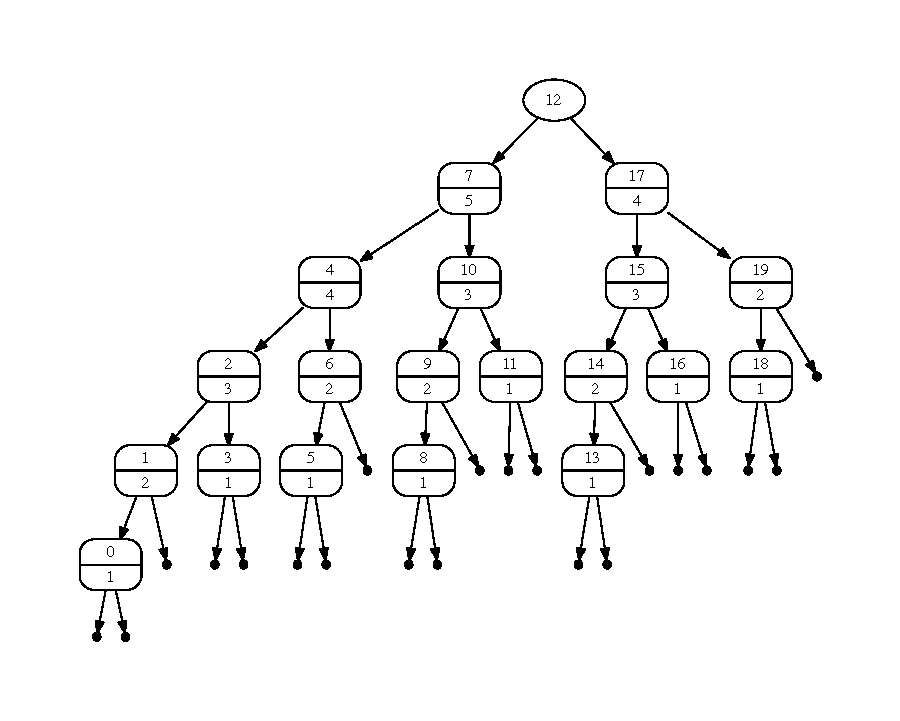
\epsfig{file=Abbildungen/avl}} 
  \caption{An AVL tree of height 6 that is as slim as possible.}
  \label{fig:avl-worst-case}
\end{figure}

\subsection{Further Reading}
In practice, 
\href{https://en.wikipedia.org/wiki/Red-black_trees}{\emph{red-black trees}} 
are slightly faster than \textsc{AVL} trees.  Similar to
\textsc{AVL} trees, a  red-black tree
  is an ordered binary tree that is approximately balanced.  Nodes are either black or red.
The children of a red node have to be black.  In order to keep red-black trees approximately
balanced, a \emph{relaxed height} of a tree is defined.  Red nodes do not contribute to the relaxed
height of a tree.  The left and right subtree of every node of a red-black tree are required to have the same 
relaxed height.  A detailed and very readable exposition of red-black trees is given by Sedgewick
\cite{sedgewick:2011}.  Red-black trees have been invented by Leonidas L.~Guibas and Robert
Sedgewick \cite{guibas:78}.



\section{Tries}
Often, the keys of a map are strings.  For example, when you search with 
\raisebox{-4pt}{
\epsfig{file=Abbildungen/google.eps, scale=0.1}}, you are using a
string as a key to lookup information that is stored in a gigantic map provided by 
\raisebox{-4pt}{
\epsfig{file=Abbildungen/google.eps, scale=0.1}}.
As another example, in an electronic phone book the keys are names and therefore are strings.  
There is a species of search trees that is particularly well adapted to the case that the keys are
strings.  These search trees are known as \href{https://en.wikipedia.org/?title=Trie}{\emph{tries}}.  
The name is derived from the word
\emph{re\underline{trie}val}.  In order that we are able to distinguish between \emph{tries} and
\emph{trees} we have to pronounce  \emph{trie}  so that it rhymes with \emph{pie}.   The data
structure of tries has been proposed 1959 by Ren\'e de la Briandais \cite{briandais:59}.

Tries are also trees, but in contrast to a binary tree where every node has two children, in a trie a
node can have as many children as there are characters in the alphabet that is used to represent the
strings.  In order to define tries formally we assume that the following is given:
\begin{itemize}
\item $\Sigma$ is finite set of \emph{characters}. $\Sigma$ is called the
      \colorbox{orange}{\emph{alphabet}}. 
\item $\Sigma^*$ is the set of all \emph{strings} that are build from the characters of $\Sigma$.
      Formally, a string is just a list of characters.  If we have $w \in \Sigma^*$, then we write $w = cr$
      if $c$ is the first letter of $w$ and if $r$ the string that remains if we remove the first
      character from $w$.
\item $\varepsilon$ denotes the empty string.
\item \textsl{Value} is the set of all the values that can be associated with the keys.  
\end{itemize}
The set $\mathbb{T}$ of all tries is defined inductively using the constructor \\[0.2cm]
\hspace*{1.3cm} 
$\texttt{Node}: \textsl{Value} \times \textsl{List}(\Sigma) \times
\textsl{List}(\mathbb{T}) \rightarrow \mathbb{T}$. 
\\[0.2cm]
The inductive definition of the set $\mathbb{T}$ has only a single clause: If
\begin{enumerate}
\item $v \in \textsl{Value} \cup \{\Omega\}$
\item $C = [c_1, \cdots, c_n] \in \textsl{List}(\Sigma)$ is a list of different characters of length
      $n$ and
\item $T = [t_1, \cdots, t_n] \in \textsl{List}(\mathbb{T})$ is a list of  tries of the same length $n$, 
\end{enumerate}
then we have 
\\[0.2cm]
\hspace*{1.3cm}  $\texttt{Node}(v, C, T) \in \mathbb{T}$.  
\\[0.2cm]
As there is only one clause in this definition, you might ask how this inductive definition gets started.
The answer is that the base case of this inductive definition is the case where
$n=0$ since in that case the lists  $C$ and $T$ are both empty.
Next, we specify the function that is represented by a trie of the form 
\\[0.2cm]
\hspace*{1.3cm} 
$\texttt{Node}(v, [c_1, \cdots, c_n], [t_1, \cdots, t_n])$.
\\[0.2cm]
In order to do so, we specify a function
\\[0.2cm]
\hspace*{1.3cm} 
$\textsl{find}: \mathbb{T} \times \Sigma^* \rightarrow \textsl{Value} \cup \{ \Omega\}$
\\[0.2cm]
that takes a trie and a string.  For a trie $t$, the expression $t.\textsl{find}(s)$ returns the
value that is associated with the string $s$ in the trie $t$.  The expression
$\texttt{Node}(v,C,T).\textsl{find}(s)$ is defined by induction on the length of the  string $s$:
\begin{enumerate}
\item $\texttt{Node}(v, C, T).\textsl{find}(\varepsilon) = v$.

      The value associated with the empty string $\varepsilon$ is stored at the root of the trie.
\item $\texttt{Node}(v, [c_1, \cdots, c_n], [t_1, \cdots, t_n]).\textsl{find}(cr) = 
        \left\{
        \begin{array}{ll}
        t_1.\textsl{find}(r) & \mbox{if} \quad c = c_1 \mbox{;} \\
        \vdots &                                     \\
        t_i.\textsl{find}(r) & \mbox{if} \quad c = c_i \mbox{;} \\
        \vdots &                                     \\
        t_n.\textsl{find}(r) & \mbox{if} \quad c = c_n \mbox{;} \\[0.2cm]
        \Omega               & \mbox{if} \quad c \notin \{c_1,\cdots,c_n\} \mbox{.}         
        \end{array}
       \right.$

      The trie $\texttt{Node}(v, [c_1, \cdots, c_n], [t_1, \cdots, t_n])$ associates a value with
      the key $cr$ if the list $[c_1, \cdots, c_n]$ has a position $i$ such that $c$ equals $c_i$
      and, furthermore, the trie  $t_i$ associates a value with the key  $r$.
\end{enumerate}

\begin{figure}[!ht]
  \centering
  \framebox{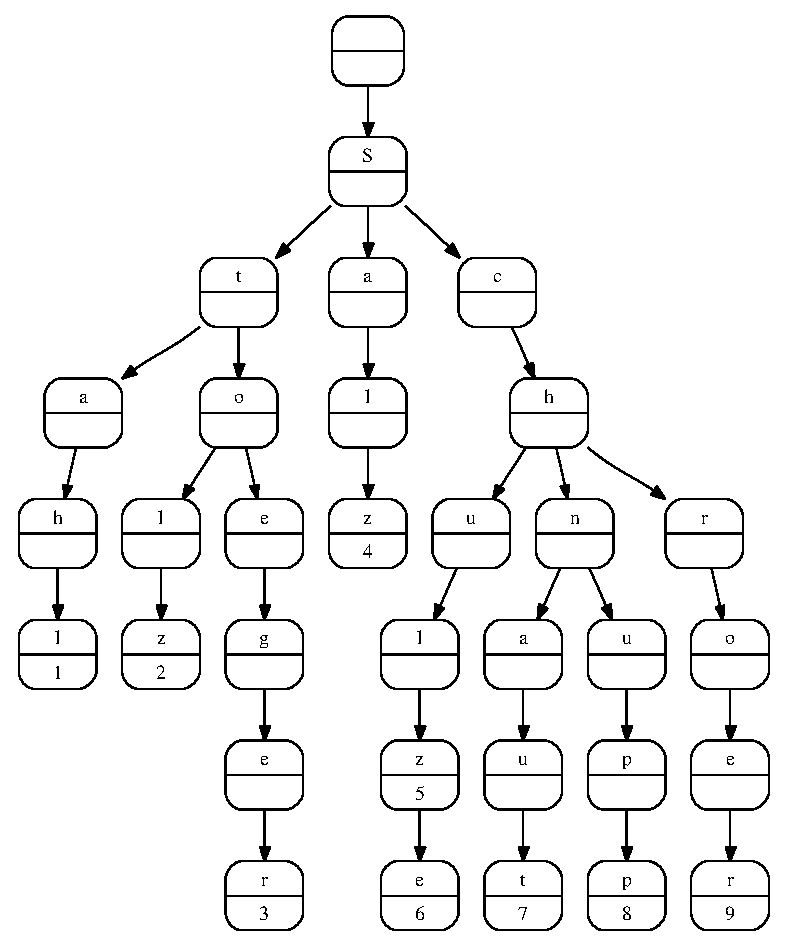
\epsfig{file=Abbildungen/trie}} 
  \caption{A trie storing some numbers.}
  \label{fig:trie}
\end{figure}

Graphically, tries are represented as trees.  Since it would be unwieldy to label the nodes of these
trees with the lists of characters corresponding to these nodes, we use a trick:  In order to
visualize a node of the form \\[0.2cm]
\hspace*{1.3cm} 
$\texttt{Node}(v, [c_1, \cdots, c_n], [t_1, \cdots, t_n])$ \\[0.2cm]
we draw a circle.  This circle is split into two parts by a horizontal line.
If the value  $v$ that is stored in this node is different from $\Omega$, then the value $v$ is
written in the lower part of the circle.  The label that we put in the upper half of the circle
depends on the parent of the node.  We will explain how this label is computed in a moment.
The node itself has $n$ different children.  These $n$ children are the tries
$t_1$, $\cdots$, $t_n$.  The node at the root of the trie $t_i$ is labeled with the character $c_i$,
i.e.~the circle that represents this node carries the label $c_i$ in its upper half.

In order to clarify these ideas, Figure  \ref{fig:trie} on page \pageref{fig:trie} shows a trie
mapping some strings to numbers.  The mapping depicted in this tree can be written as a functional
relation: 
\\[0.2cm]
\hspace*{1.3cm} $ \bigl\{ \langle \textrm{``Stahl''},   1  \rangle, \langle \textrm{``Stolz''},     2  \rangle, \langle \textrm{``Stoeger''},   3  \rangle, 
             \langle \textrm{``Salz''},      4  \rangle, \langle \textrm{``Schulz''},    5  \rangle$, \\[0.2cm]
\hspace*{1.5cm} $\langle \textrm{``Schulze''},   6  \rangle, \langle \textrm{``Schnaut''},   7  \rangle, 
  \langle \textrm{``Schnupp''},   8  \rangle, 
  \langle \textrm{``Schroer''},   9  \rangle\}$. \\[0.2cm]
Since the node at the root has no parent, the upper half of  the circle representing the root is
empty.  The lower half of  this circle is empty because the trie doesn't associate a value with the
empty string.  This root node corresponds to the term 
\\[0.2cm]
\hspace*{1.3cm}
 $\texttt{Node}(\Omega,[\textrm{`S'}], [t])$. 
\\[0.2cm]
Here,  $t$ denotes the trie that is labeled with the character  ``S'' at its root.
This trie can then be represented by the term  \\[0.2cm]
\hspace*{1.3cm} 
$\texttt{Node}(\Omega,[\textrm{`t'},\textrm{`a'},\textrm{`c'}], [t_1, t_2, t_3])$. \\[0.2cm]
This trie has three children that are labeled with the characters  ``t'', ``a'', and ``c''.

\subsection{Insertion in Tries}
Next, we present formul\ae\ that describe how new values can be inserted into an existing tries,
i.e.~we specify the method \texttt{insert}.  The signature of \texttt{insert} is given as follows:
\\[0.2cm]
\hspace*{1.3cm}
$\textsl{insert}: \mathbb{T} \times \Sigma^* \times \textsl{Value} \rightarrow \mathbb{T}$.
\\[0.2cm]
The result of evaluating \\[0.2cm]
\hspace*{1.3cm} 
$\texttt{Node}(v_1, [c_1, \cdots, c_n], [t_1, \cdots, t_n]).\textsl{insert}(w, v_2)$
\\[0.2cm]
for a string $w\in \Sigma^*$ and a value $v_2 \in \textsl{Value}$ is defined by induction on the
length of $w$.
\begin{enumerate}
\item $\texttt{Node}(v_1,L,T).\textsl{insert}(\varepsilon, v_2) = \texttt{Node}(v_2,L,T)$,
  
      If a new value $v_2$ is associated with the empty string $\varepsilon$, then the old value
      $v_1$, that had been stored at the root before, is overwritten.
\item $\texttt{Node}\bigl(v_1,[c_1,\cdots,c_i,\cdots,c_n], [t_1,\cdots,t_i,\cdots,t_n]\bigr).\textsl{insert}(c_ir,v_2) =$ \\[0.2cm]
      \hspace*{1.3cm}  
      $\texttt{Node}\bigl(v_1,[c_1,\cdots,c_i,\cdots,c_n], [t_1,\cdots,t_i.\textsl{insert}(r,v_2),\cdots,t_n]\bigr)$.

      In order to associate a value $v_2$ with the string $c_ir$ in the trie
      \\[0.2cm]
      \hspace*{1.3cm}
      $\texttt{Node}\bigl(v_1,[c_1,\cdots,c_i,\cdots,c_n], [t_1,\cdots,t_i,\cdots,t_n]\bigr)$ 
      \\[0.2cm]
      we have to recursively associate the value $v_2$ with the string $r$ in the trie $t_i$.
\item $c \not\in\{c_1,\cdots,c_n\} \;\rightarrow\;\texttt{Node}\bigl(v_1,[c_1,\cdots,c_n], [t_1,\cdots,t_n]\bigr).\textsl{insert}(cr,v_2) =$ \\[0.2cm]
      \hspace*{1.3cm}  
      $\texttt{Node}\bigl(v_1,[c_1,\cdots,c_n,c], [t_1,\cdots,t_n,\texttt{Node}(\Omega,[],[]).\textsl{insert}(r,v_2)]\bigr)$.
      
      If we want to associate a value $v$ with the key $cr$ in the trie
      $\texttt{Node}\bigl(v_1,[c_1,\cdots,c_n], [t_1,\cdots,t_n]\bigr)$ then, if the character $c$
      does not occur in the list $[c_1,\cdots,c_n]$, we first have to create a new empty trie.
      This trie has the form \\[0.2cm]
      \hspace*{1.3cm} $\texttt{Node}(\Omega, [], [])$. \\[0.2cm]
      Next, we associate the value $v_2$ with the key $r$ in this empty trie.  Finally,
      we append the character $c$ to the end of the list $[c_1,\cdots,c_n]$ and append the trie
        \\[0.2cm] 
      \hspace*{1.3cm}
      $\texttt{Node}(\Omega, [], []).\textsl{insert}(r,v_2)$ 
      \\[0.2cm]
      to the end of the list $[t_1,\cdots,t_n]$.
\end{enumerate}

\subsection{Deletion in Tries}
Finally, we present formul\ae\ that specify how a key can be deleted from a trie.
To this end, we define the auxiliary function
\\[0.2cm]
\hspace*{1.3cm} 
$\textsl{isEmpty}: \mathbb{T} \rightarrow \mathbb{B}$.
\\[0.2cm]
For a trie $t$, we have $t.\textsl{isEmpty}() = \mathtt{true}$ if and only if the trie $t$ does not
store any key.  The following formul\ae\ specify the function \textsl{isEmpty}:
\begin{enumerate}
\item $\texttt{Node}(\Omega, [],[]).\textsl{isEmpty}() = \mathtt{true}$,
\item $v \not= \Omega \rightarrow 
       \texttt{Node}(v, [c_1,\cdots,c_n],[t_1,\cdots,t_n]).\textsl{isEmpty}() = \mathtt{false}$,
\item $\texttt{Node}(\Omega, L, T).\textsl{isEmpty}() = \textsl{isEmptyList}(T)$
\end{enumerate}
In the last formula we have used the auxiliary function
\\[0.2cm]
\hspace*{1.3cm}
$\textsl{isEmptyList}: \textsl{List}(\mathbb{T}) \rightarrow \mathbb{B}$.
\\[0.2cm]
For a list of tries, this function checks whether all tries in this list are empty.  Formally,
$\textsl{isEmptyList}(l)$ is defined by induction on the length of the list $l$.
\begin{enumerate}
\item $\textsl{isEmptyList}\bigl([]\bigr) = \mathtt{true}$,
\item $\textsl{isEmptyList}\bigl([t] + r\bigr) = \bigl(t.\textsl{isEmpty}() \wedge \textsl{isEmptyList}(r)\bigr)$,

      because all  tries in the list $[t]+r$ are empty if  $t$ is an empty trie
      and, furthermore, all tries in  $r$ are empty.
\end{enumerate}
Now, we can specify the method
\\[0.2cm]
\hspace*{1.3cm}
$\textsl{delete}: \mathbb{T} \times \Sigma^* \rightarrow \mathbb{T}$.
\\[0.2cm]
For a trie  $t \in \mathbb{T}$ and a string $w \in \Sigma^*$ the value of
 \\[0.2cm]
\hspace*{1.3cm} 
$t.\textsl{delete}(w)$
\\[0.2cm]
is defined by induction on the length of  $w$.
\begin{enumerate}
\item $\texttt{Node}(v,L,T).\textsl{delete}(\varepsilon) = \texttt{Node}(\Omega,L,T)$

      The value that is associated with the empty  string $\varepsilon$ is stored at the root of the
      trie where is can be deleted without further ado.
\item $\begin{array}[t]{ll}
       t_i.\textsl{delete}(r).\textsl{isEmpty}()   & \rightarrow \\
       \texttt{Node}(v, [c_1,\cdots,c_i,\cdots,c_n],[t_1,\cdots,t_i,\cdots,t_n]).\textsl{delete}(c_ir) 
       & = \\
       \qquad 
       \texttt{Node}(v, [c_1,\cdots,c_{i-1},c_{i+1},\cdots,c_n],[t_1,\cdots,t_{i-1},t_{i+1},\cdots,t_n]).
       \end{array}
       $

       If  the key that is to be deleted starts with the character $c_i$ and if deletion of  the key
       $r$ in the $i$th  trie $t_i$ yields an empty
       trie, then both the $i$th character $c_i$ and the $i$th trie $t_i$ are deleted.
\item $\begin{array}[t]{ll}
       \neg t_i.\textsl{delete}(r).\textsl{isEmpty}()   & \rightarrow \\
       \texttt{Node}(v, [c_1,\cdots,c_i,\cdots,c_n],[t_1,\cdots,t_i,\cdots,t_n]).\textsl{delete}(c_ir) 
       & = \\
       \qquad \texttt{Node}(v, [c_1,\cdots,c_i,\cdots,c_n],[t_1,\cdots,t_i.\textsl{delete}(r),\cdots,t_n]).
       \end{array}
       $

       If  the key that is to be deleted starts with the character $c_i$ and if deletion of  the key
       $r$ in the $i$th  trie $t_i$ yields a non-empty trie, then the key $r$ has to be deleted recursively
       in the trie $t_i$.
\item $c \notin C \rightarrow \texttt{Node}(v, C, T).\textsl{delete}(cr) =
       \texttt{Node}(v, C, T)$. 
       
       If  the key that is to be deleted starts with the character $c$ and if $c$ does not occur in
       the list of characters $C$, then the trie does not contain the key $cr$ and therefore there
       is nothing  to do:  The trie is left unchanged.
\end{enumerate}

\subsection{Complexity}
It is straightforward to see that the complexity of looking up the value associated with a string
$s$ of length $k$ is $\Oh(k)$.  In particular, it is independent on the number of strings $n$.  As
it is obvious that we have to check all $k$ characters of the string $s$, this bound can not be
improved.   Another advantage of tries is the fact that they use very little storage to store the
keys because common prefixes are only stored once. 

\subsection{Implementing Tries in \textsc{SetlX}}
\begin{figure}[!ht]
\centering
\begin{Verbatim}[ frame         = lines, 
                  framesep      = 0.3cm, 
                  firstnumber   = 1,
                  labelposition = bottomline,
                  numbers       = left,
                  numbersep     = -0.2cm,
                  xleftmargin   = 0.8cm,
                  xrightmargin  = 0.8cm,
                ]
    class map() {
        mValue := om;
        mChars := [];
        mTries := [];
    
      static {
        find    := procedure(s)    { ... };
        insert  := procedure(s, v) { ... };
        delete  := procedure(s)    { ... };
        isEmpty := procedure()     { ... };
      }
    }
\end{Verbatim}
\vspace*{-0.3cm}
\caption{Outline of the class \texttt{trieMap}.}
\label{fig:trie.stlx-outline}
\end{figure}

\noindent
We proceed to discuss the implementation of tries.  Figure \ref{fig:trie.stlx-outline} shows the
outline of the class \texttt{trie}.  This class supports three member variables.  In order to
understand these member variables, remember that a trie has the form
\\[0.2cm]
\hspace*{1.3cm}
$\texttt{Node}(v, C, T)$
\\[0.2cm]
where $v$ is the value stored at the root, $C$ is the list of characters, and $t$ is a list of
tries.  Therefore, the member variables have the following semantics:
\begin{enumerate}
\item \texttt{mValue} represent the value $v$ stored at the root of this trie,  
\item \texttt{mChars} represent the list  $C$ of characters.  If there is a string $cr$ such that
      the trie stores a value associated with this string, then the character $c$ will be an element of
      the list $C$.
\item \texttt{mTries} represent the list of subtries $T$.  
\end{enumerate}
The class \texttt{trieMap} implements the abstract data type \texttt{map} and therefore provides the
methods \texttt{find}, \texttt{insert}, and \texttt{delete}.  Furthermore, the method
\texttt{isEmpty} is an auxiliary method that is needed in the implementation of the method 
\texttt{delete}.  This method checks whether the given trie corresponds to the empty map.  The
implementation of all these methods is given below. 

\begin{figure}[!ht]
\centering
\begin{Verbatim}[ frame         = lines, 
                  framesep      = 0.3cm, 
                  firstnumber   = 1,
                  labelposition = bottomline,
                  numbers       = left,
                  numbersep     = -0.2cm,
                  xleftmargin   = 0.8cm,
                  xrightmargin  = 0.8cm,
                ]
    find := procedure(s) {
        match (s) {
            case ""   : return mValue;
            case [c|r]: for (i in [1 .. #mChars]) {
                            if (mChars[i] == c) {
                                return mTries[i].find(r);
                            }
                        }
                        return;  // not found
        }
    };
\end{Verbatim}
\vspace*{-0.3cm}
\caption{Implementation of \texttt{find} for tries.}
\label{fig:trie.stlx-find}
\end{figure}

The method \texttt{find} takes a string $s$ as its sole argument and checks whether the given trie
contains a value associated with the string $s$.  Essentially, the are two cases:
\begin{enumerate}
\item If $s$ is the empty string, the value associated with $s$ is stored in the member variable
      \texttt{mValue} at the root of this trie.
\item Otherwise, $s$ can be written as $s = cr$ where $c$ is the first character of $s$ while $r$
      consists of the remaining characters.  In order to check whether the trie has a value stored
      for $s$ we first have to check whether there is an index $i$ such that \texttt{mChars[$i$]} is
      equal to $c$.  If this is the case, the subtrie \texttt{mTries[$i$]} contains the value
      associated with $s$.  Then, we have to invoke \texttt{find} recursively on this subtrie.

      If the loop in line 4 does not find the character $c$ in the list \texttt{mChars}, then the method
      \texttt{find} will just return \texttt{om} in line 9.
\end{enumerate}


\begin{figure}[!ht]
\centering
\begin{Verbatim}[ frame         = lines, 
                  framesep      = 0.3cm, 
                  firstnumber   = 1,
                  labelposition = bottomline,
                  numbers       = left,
                  numbersep     = -0.2cm,
                  xleftmargin   = 0.8cm,
                  xrightmargin  = 0.8cm,
                ]
    insert := procedure(s, v) {
        match (s) {
            case ""   : this.mValue := v;
            case [c|r]: for (i in [1 .. #mChars]) {
                            if (mChars[i] == c) {
                                t := mTries[i];
                                t.insert(r,v);
                                this.mTries[i] := t;
                                return;
                            }
                        }
                        newTrie := trieMap();
                        newTrie.insert(r, v);
                        this.mChars += [ c ]; 
                        this.mTries += [ newTrie ];
        } 
    };
\end{Verbatim}
\vspace*{-0.3cm}
\caption{Implementation of \texttt{insert} for tries.}
\label{fig:trie.stlx-insert}
\end{figure}


The method \texttt{insert} takes a string $s$ and an associated value $v$ that is to be inserted
into the given trie.  The implementation of \texttt{insert} works somewhat similar to the
implementation of \texttt{find}.
\begin{enumerate}
\item If the string $s$ is empty, then the value $v$ has to be positioned at the root of this trie.
      Hence we just set \texttt{mValue} to $v$.
\item Otherwise, $s$ can be written as $cr$ where $c$ is the first character of $s$ while $r$
      consists of the remaining characters.  In this case, we need to check whether the list
      \texttt{mChars} already contains the character $c$ or not.
      \begin{enumerate}
      \item If $c$ is the $i$-th character of \texttt{mChars}, then we have to insert the value $v$
            in the trie \texttt{mTries[$i$]}.  However, this is a little tricky to do.
            First, we retrieve the subtrie \texttt{mTries[$i$]} and store this trie into the
            variable $t$.  Next, we can insert the value $v$ into the trie $t$ using the rest $r$ of the
            string $s$ as the key.  Finally, we have to set \texttt{mTries[$i$]} to $t$.  At this point, you
            might wonder why we couldn't have just used the statement
            \\[0.2cm]
            \hspace*{1.3cm}
            \texttt{this.mTries[i].insert(r,v);}
            \\[0.2cm]
            to achieve the same effect. Unfortunately, this does not work because the expression \texttt{this.mTries[i]} will
            create a temporary value and inserting $v$ into this temporary value will not change the
            original list \texttt{mTries}.
       \item If $c$ does not occur in \texttt{mChars}, things are straightforward: We create a new
             empty trie and insert $v$ into this trie.  Next, we append the character $c$ to
             \texttt{mChars} and simultaneously append the newly created trie that contains $v$ to
             \texttt{mTries}. 
      \end{enumerate}
\end{enumerate}

\begin{figure}[!ht]
\centering
\begin{Verbatim}[ frame         = lines, 
                  framesep      = 0.3cm, 
                  firstnumber   = 1,
                  labelposition = bottomline,
                  numbers       = left,
                  numbersep     = -0.2cm,
                  xleftmargin   = 0.0cm,
                  xrightmargin  = 0.0cm,
                ]
    delete := procedure(s) {
        match (s) {
            case ""   : this.mValue := om;
            case [c|r]: 
                for (i in [1 .. #mChars]) {
                     if (mChars[i] == c) {
                         t := mTries[i]; 
                         t.delete(r);
                         this.mTries[i] := t;
                         if (this.mTries[i].isEmpty()) {
                             this.mChars := removeIthElement(mChars, i);
                             this.mTries := removeIthElement(mTries, i);
                         }
                         return;
                     }
                }
        }
    };
\end{Verbatim}
\vspace*{-0.3cm}
\caption{Implementation of \texttt{delete} for tries.}
\label{fig:trie.stlx-delete}
\end{figure}

The method \texttt{delete} takes a string and, provided there is a value associated with $s$, this
value is deleted,
\begin{enumerate}
\item If the string $s$ is empty, the value associated with $s$ is stored at the root of this trie.
      In order to remove this value, the variable \texttt{mValue} is set to \texttt{om}.
\item Otherwise, $s$ can be written as $cr$ where $c$ is the first character of $s$ while $r$
      consists of the remaining characters.  In this case, we need to check whether the list
      \texttt{mChars} contains the character $c$ or not.
 
      If $c$ is the $i$-th character of \texttt{mChars}, then we have to delete the value 
      associated with $r$ in the trie \texttt{mTries[$i$]}.  Again, this is tricky to do.
      First, we retrieve the subtrie \texttt{mTries[$i$]} and store this trie into the
      variable $t$.  Next, the value associated with $r$ is deleted in $t$ and, finally, 
      $t$ is written to \texttt{mTries[$i$]}.  

      After the deletion, the subtrie  \texttt{mTries[$i$]} might well be empty.  In this case,
      we remove the $i$-th character form \texttt{mChars} and also remove the $i$-th trie from the list
      \texttt{mTries}.  This is done with the help of the function \texttt{removeIthElement},
      which is shown in Figure \ref{fig:trie.stlx-removeIthElement}.
\end{enumerate}

\begin{figure}[!ht]
\centering
\begin{Verbatim}[ frame         = lines, 
                  framesep      = 0.3cm, 
                  firstnumber   = 1,
                  labelposition = bottomline,
                  numbers       = left,
                  numbersep     = -0.2cm,
                  xleftmargin   = 0.8cm,
                  xrightmargin  = 0.8cm,
                ]
    isEmpty := procedure() {
        return mValue == om && mChars == [];
    };
\end{Verbatim}
\vspace*{-0.3cm}
\caption{Implementation of \texttt{isEmpty} for tries.}
\label{fig:trie.stlx-isEmpty}
\end{figure}

In order to check whether a given trie is empty we have to check that no value is stored at the root
and that the list \texttt{mChars} is empty, since then the list \texttt{mTries} will also be empty.

\begin{figure}[!ht]
\centering
\begin{Verbatim}[ frame         = lines, 
                  framesep      = 0.3cm, 
                  firstnumber   = 1,
                  labelposition = bottomline,
                  numbers       = left,
                  numbersep     = -0.2cm,
                  xleftmargin   = 0.8cm,
                  xrightmargin  = 0.8cm,
                ]
    removeIthElement := procedure(l, i) {
        return l[1 .. i-1] + l[i+1 .. #l];
    };
\end{Verbatim}
\vspace*{-0.3cm}
\caption{The function to remove the $i$-th element from a list.}
\label{fig:trie.stlx-removeIthElement}
\end{figure}

Finally, the implementation of \texttt{removeIthElement}, which is shown in Figure
\ref{fig:trie.stlx-removeIthElement}, is straightforward. 


\exercise
\textbf{Binary Tries}:  Let us assume that our alphabet is the binary alphabet, i.e.~the alphabet
only contains the two digits $0$ and $1$.  Therefore we have $\Sigma = \{0,1\}$.  Every natural
number can be regarded as a string from the alphabet $\Sigma$, so that numbers are effectively
elements of $\Sigma^*$.  The set $\BT$ of \colorbox{orange}{\emph{binary tries}} is defined by induction:
\begin{enumerate}
\item $\textsl{Nil} \in \BT$.
\item $\textsl{Bin}(v,l,r) \in \BT$ provided that
      \begin{enumerate}
      \item $v \in \textsl{Value} \cup \{\Omega\}$ \quad and
      \item $l,r \in \BT$.
      \end{enumerate}
\end{enumerate}
The semantics of binary tries is fixed by defining the function
\\[0.2cm]
\hspace*{1.3cm}
$\textsl{find}: \BT \times \mathbb{N} \rightarrow \textsl{Value} \cup \{ \Omega \}$.
\\[0.2cm]
Given a binary trie $b$ and a natural number $n$, the expression
\\[0.2cm]
\hspace*{1.3cm}
$b.\textsl{find}(n)$ 
\\[0.2cm]
returns the value in $b$ that is associated with the number $n$.  If there is no value associated
with $b$, then the expression evaluates to $\Omega$.  Formally, the value of the expression
 $b.\textsl{find}(n)$ is defined by in duction on $b$.  The induction step requires a side induction
 with respect to $n$.
\begin{enumerate}
\item $\textsl{Nil}.\textsl{find}(n) = \Omega$,

      since the empty trie doesn't store any values.
\item $\textsl{Bin}(v,l,r).\textsl{find}(0) = v$,

      because $0$ is interpreted as the empty string $\varepsilon$.
\item $\textsl{Bin}(v,l,r).\textsl{find}(2\cdot n + 2) = l.\textsl{find}(n)$,

      because if a number is represented in binary, then the last bit of every even number is zero
      and zero chooses the left subtree.
\item $\textsl{Bin}(v,l,r).\textsl{find}(2 \cdot n + 1) = r.\textsl{find}(n)$,

      because if a number is represented in binary, then the last bit of every odd number is 1 and 
      1 is associated with the right subtree.
\end{enumerate}
Solve the following exercises:
\begin{enumerate}[(a)]
\item Provide equations that specify the methods \texttt{insert} and \texttt{delete} in a binary trie.
      When specifying delete you should take care that empty binary trees are reduced to
      $\textsl{Nil}$.

      \textbf{Hint}:  It might be helpful to provide an auxiliary method that simplify those binary
      tries that are empty.
\item Implement binary tries in \textsc{SetlX}.
\end{enumerate}
\textbf{Remark}: Binary tries are known as \emph{digital search trees}.  \eox

\section{Hash Tables}
It is very simple to implement a function of the form \\[0.2cm]
\hspace*{1.3cm} $f: \textsl{Key} \rightarrow \textsl{Value}$ \\[0.2cm]
provided the set \textsl{Key} is a set of natural numbers of the form  \\[0.2cm]
\hspace*{1.3cm} $\textsl{Key} = \{ 1, 2, \cdots, n \}$. \\[0.2cm]
In this case, we can implement the function $f$ via an array of size $n$.
Figure \ref{fig:map-array.stlx} shows how a map can be realized in this case.

\begin{figure}[!ht]
\centering
\begin{Verbatim}[ frame         = lines, 
                  framesep      = 0.3cm, 
                  firstnumber   = 1,
                  labelposition = bottomline,
                  numbers       = left,
                  numbersep     = -0.2cm,
                  xleftmargin   = 0.8cm,
                  xrightmargin  = 0.8cm,
                ]
    class map(n) {
        mArray := [1..n];
      static {
        find   := k |-> mArray[k];
        insert := procedure(k, v) { this.mArray[k] := v;  };
        delete := procedure(k)    { this.mArray[k] := om; };
        f_str  := procedure()     { return str(mArray);   };
      }
    }
\end{Verbatim}
\vspace*{-0.3cm}
\caption{Implementing a map as an array.}
\label{fig:map-array.stlx}
\end{figure}




If the domain $D := \textsl{dom}(f)$ of the function $f$ is not a set of the form $\{1, \cdots, n\}$, 
then we can instead try to find a one-to-one mapping of $D$ onto a set of the form $\{1,\cdots,n\}$.
Let us explain the idea with a simple example:  Suppose we wanted to implement a telephone
dictionary.
To simplify things, let us assume first that all the names stored in our telephone dictionary
have a length of 8 characters.  To achieve this, names that are shorter than eight characters
are filled with spaces and if a name has more than eight characters, all characters after the
eighth character are dropped.

Next, every name is translated into an index.  In order to do so, the different
characters are interpreted as digits in a system where the digits can take values starting
from 0 up to the value 26.
Let us assume that the function  $\textsl{ord}$ takes a character from the set
\\[0.2cm]
\hspace*{1.3cm}
$\Sigma = \{ \texttt{' '}, \texttt{'a'}, \texttt{'b'}, \texttt{'c'}, \cdots, \texttt{'x'}, \texttt{'y'}, \texttt{'z'} \}$ 
\\[0.2cm]
and assigns a number from the set $\{0,\cdots,26\}$ to this character, i.e.~we have \\[0.2cm]
\hspace*{1.3cm} 
$\textsl{ord}: \{ \texttt{' '}, \texttt{'a'}, \texttt{'b'}, \texttt{'c'}, \cdots, \texttt{'x'}, \texttt{'y'}, \texttt{'z'} \} \rightarrow \{0,\cdots, 26\}$.
\\[0.2cm]
Then, the value of the string  $w = c_0c_1\cdots c_7$ can be computed by the function \\[0.2cm]
\hspace*{1.3cm} 
$\textsl{code}: \Sigma^* \rightarrow \mathbb{N}$ \\[0.2cm]
as follows: \\[0.2cm]
\hspace*{1.3cm} 
$\textsl{code}(c_0c_1\cdots c_7) = 1 + \sum\limits_{i=0}^7 \textsl{ord}(c_i) \cdot 27^i$.
\\[0.2cm]
Then, the function \textsl{code} maps the set of all non-empty strings with at most eight characters in a
one-to-one way to the set of numbers $\{1,\cdots,27^8\}$.


\begin{figure}[!ht]
  \centering
  \framebox{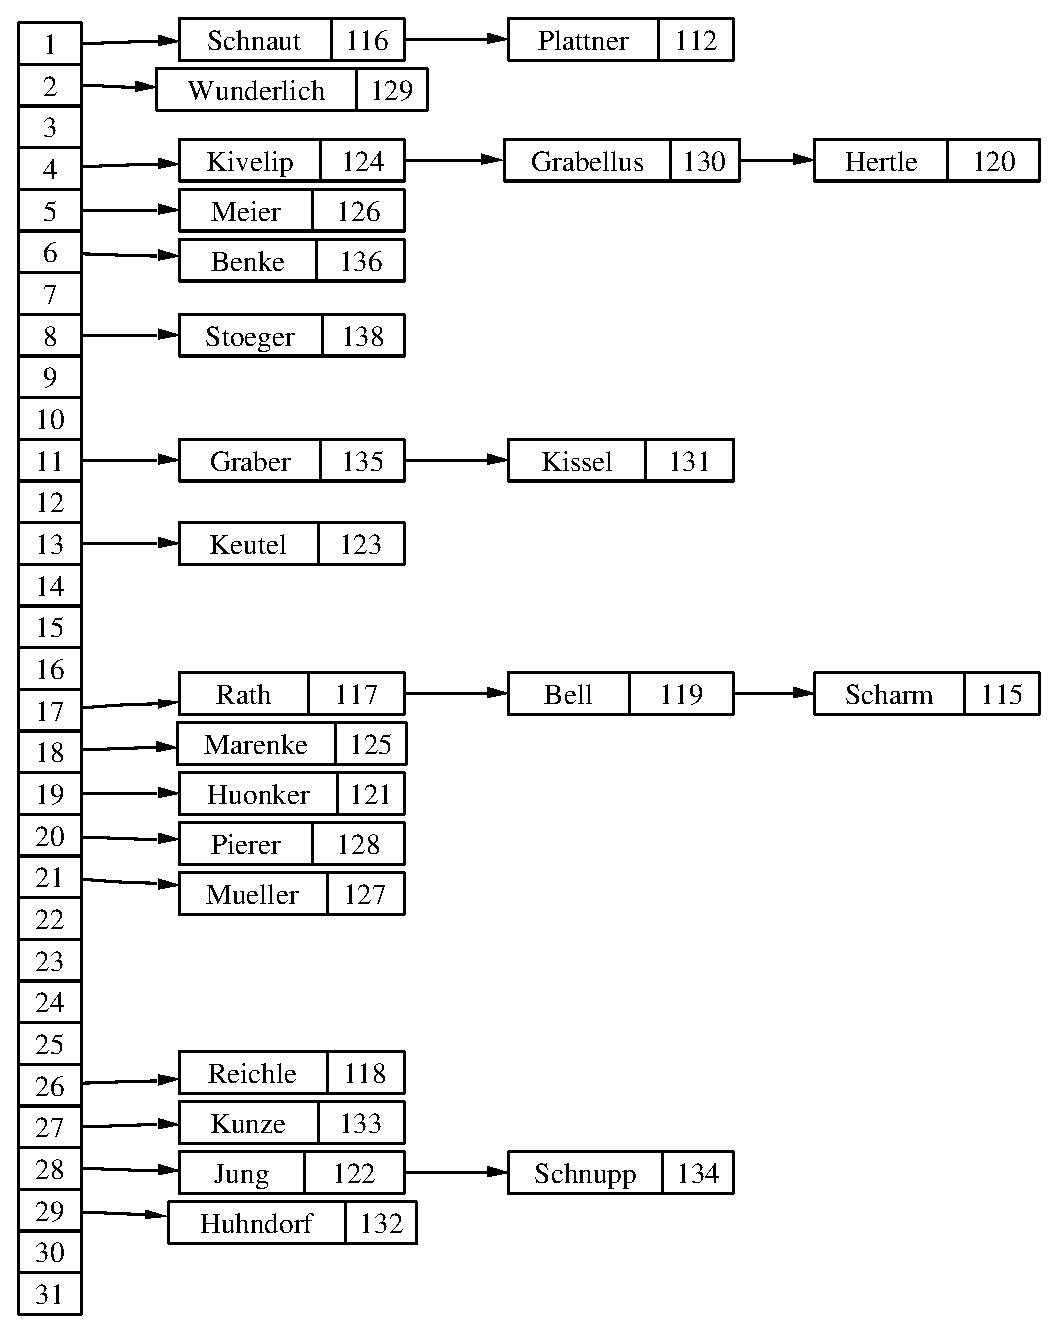
\epsfig{file=Abbildungen/hash-table,scale=0.6}} 
  \caption{Eine Hash-Tabelle}
  \label{fig:hash-example}
\end{figure}

\noindent
Unfortunately, this naive implementation has several problems: 
\begin{enumerate}
\item The array needed to store the telephone dictionary has a size of 
      \\[0.2cm]
      \hspace*{1.3cm} $27^8 = 282\,429\,536\,481$ \\[0.2cm]
      entries.  Even if every entry only needs 8 bytes, we still would need more than one terabyte
      of memory.
\item If two names happen to differ only after their eighth character, then we would not be able to
      store both of theses names as we would not be able to distinguish these names.
\end{enumerate}
These problems can be solved as follows:
\begin{enumerate}
\item We have to change the function  \texttt{code} so that the result of this function is always
      less than or equal to some given number \texttt{size}.  Here, the number \texttt{size} specifies
      the number of entries of the array that we intend to use.  This number will be in the same
      order of magnitude as the number of key-value pairs that we want to store in our dictionary.

      There is a simple way to adapt the function  \textsl{code} so that its result is never bigger
      than a given number \texttt{size}: If we define \textsl{code} as
      \\[0.2cm]
      \hspace*{1.3cm} 
      $\textsl{code}(c_0c_1\cdots c_n) = \left(\sum\limits_{i=0}^n \textsl{ord}(c_i) \cdot
        27^i\right) \;\%\; \texttt{size} + 1$,
      \\[0.2cm]
      then we will always have $\textsl{code}(c_0c_1\cdots c_n) \leq \mathtt{size}$.  In order to
      prevent overflows we can define the partial sum $s_k$ for  $k=n,n-1,\cdots,1,0$ by induction:
      \begin{enumerate}
      \item $s_n = \textsl{ord}(c_n)$,
      \item $s_{k} = \bigl(\textsl{ord}(c_{k}) + s_{k+1} \cdot 27 \bigr) \;\%\; \texttt{size}$.
      \end{enumerate}
      Then we have
      \hspace*{1.3cm} 
      $s_0 + 1 = \left(\sum\limits_{i=0}^n \textsl{ord}(c_i) \cdot 27^i\right) \;\%\; \texttt{size} + 1$.
\item Rather than storing the values associated with the keys in an array, the values are now stored
      in linked lists that contain key-value pairs.  The array only stores pointers to these linked list.
      
      The reason we have to use linked lists is the fact that different keys may be mapped to the
      same index.  Hence, we can no longer store the values directly in the array.  Instead,
      the values of all keys that map to the same index are stored in a
      linked list of key-value pairs.  These linked lists are then stored in the array.  As long as
      these lists contain only a few entries, the look-up of a key is still fast: Given a key $k$,
      we first compute 
      \\[0.2cm]
      \hspace*{1.3cm}
      $\mathtt{idx} = \textsl{code}(k)$.
      \\[0.2cm]
      Then, \texttt{array[idx]} returns a linked list containing a pair of the form $\langle k, v \rangle$.
      In order to find the value associated with the key $k$ we have to search this list for the key
      $k$.
\end{enumerate}
Figure \ref{fig:hash-example} on page \pageref{fig:hash-example} shows an array that contains
linked lists.  An array of this kind is called a
\href{https://en.wikipedia.org/wiki/Hash_table}{\emph{hash table}}.
We proceed to discuss the implementation of hash tables in \textsc{Setlx}.



\begin{figure}[!ht]
  \centering
\begin{Verbatim}[ frame         = lines, 
                  framesep      = 0.3cm, 
                  labelposition = bottomline,
                  numbers       = left,
                  numbersep     = -0.2cm,
                  xleftmargin   = 0.0cm,
                  xrightmargin  = 0.0cm
                ]
    class hashTable(n) {
        mSize    := n;
        mEntries := 0;  // number of entries
        mArray   := [ {} : i in [1 .. mSize] ];
        mAlpha   := 2;  // load factor
    
        static {
            sOrd    := { [ char(i), i ] : i in [ 0 .. 127 ] };
            sPrimes := [ 3, 7, 13, 31, 61, 127, 251, 509, 1021, 2039, 
                         4093, 8191, 16381, 32749, 65521, 131071, 
                         262139, 524287, 1048573, 2097143, 4194301, 
                         8388593, 16777213, 33554393, 67108859, 
                         134217689, 268435399, 536870909, 1073741789, 
                         2147483647 
                       ];    
            hashCode := procedure(s)          { ... };
            find     := procedure(key)        { ... };
            insert   := procedure(key, value) { ... };
            rehash   := procedure()           { ... };
            delete   := procedure(key)        { ... };    
        }
    }
\end{Verbatim}
\vspace*{-0.3cm}
  \caption{Outline of the class \texttt{hashTable}.}
  \label{fig:hashTable.stlx-outline}
\end{figure}

Figure \ref{fig:hashTable.stlx-outline} shows the outline of the class \texttt{hashTable}.  
\begin{enumerate}
\item The constructor is called with one argument.  This argument $n$ is the initial size
      of the array storing the different key-value lists.  The constructor constructs an empty hash
      table with the given capacity.
\item \texttt{mSize} is the actual size of the array that stores the different key-value lists.
      Although this variable is initialized as $n$, it can later be increased.  This happens
      if the hash table becomes overcrowded.
\item \texttt{mEntries} is the number key-value pairs that are stored in this hash map.
      Since, initially, this map is entry, \texttt{mEntries} is  initialized as $0$.
\item \texttt{mArray} is the array containing the list of key value pairs.

      In our implementation, the key-value pairs are not stored in a list but, instead, they are
      stored in a set.  Since every key is associated with at most one value, this set can be interpreted as a
      functional relation.  Therefore, looking up a key is more efficient than it would be if we had
      used a list.  Although we actually use a relation instead of a list, we will still call
      this relation the \emph{list of key-value pairs}.

      As the hash map is initially empty, all entries of \texttt{mArray} are initialized as empty sets.
\item \texttt{mAlpha} is the \emph{load factor} of our hash table.  If at any point in time, we have
      \\[0.2cm]
      \hspace*{1.3cm}
      $\texttt{mEntries} > \texttt{mAlpha} \cdot \texttt{mSize}$,
      \\[0.2cm]
      then we consider our hash table to be \emph{overcrowded}.  In that case, we increase the size
      of the array \texttt{mArray}.  To determine the best value for \texttt{mAlpha}, we have to
      make a tradeoff:  If \texttt{mAlpha} were too big, many entries in the array \texttt{mArray}
      would be empty and thus we would waste space.  On the other hand, if \texttt{mAlpha} were too
      small, the key-value lists would become very long and hence it would take too much time to
      search for a given key in one of these lists.
\item Our implementation maintains two static variables.
  \begin{enumerate}
  \item \texttt{sOrd} is a functional relation mapping characters to \textsc{Ascii} codes.
        This relation is needed for the efficient computation of the method \texttt{hashCode}
        discussed below.

        In \texttt{SetlX} there is no function that returns the \textsc{Ascii} code of a given character.
        Fortunately, it is easy to implement this function as a binary relation via the function
        $\mathtt{char}(i)$.  Given a number $i \in \{0,\cdots,127\}$, the function $\mathtt{char}(i)$
        returns the character that has \textsc{Ascii} code $i$.  The relation \texttt{sOrd} is the inverse
        of the function \texttt{char}.
  \item \texttt{sPrimes} is a list of prime numbers.  Roughly, these prime numbers double in size.
        The reason is that performance of a hash table is best if the size of \texttt{mArray} is a
        prime number.  When \texttt{mArray} gets overcrowded, the idea is to, more or less, double
        the size of \texttt{mArray}.  To achieve this, the variable \texttt{sPrimes} is needed.
  \end{enumerate}
\end{enumerate}
Next, we discuss the implementation of the various methods.

\begin{figure}[!ht]
\centering
\begin{Verbatim}[ frame         = lines, 
                  framesep      = 0.3cm, 
                  firstnumber   = 1,
                  labelposition = bottomline,
                  numbers       = left,
                  numbersep     = -0.2cm,
                  xleftmargin   = 0.0cm,
                  xrightmargin  = 0.0cm,
                ]
        hashCode := procedure(s) {
            return hashCodeAux(s) + 1;
        };
        hashCodeAux := procedure(s) {
            if (s == "") {
                return 0;
            }
            return (sOrd[s[1]] + 128 * hashCodeAux(s[2..])) % mSize;
        };
\end{Verbatim}
\vspace*{-0.3cm}
\caption{Implementation of the method \texttt{hashCode}.}
\label{fig:hashTable.stlx-hashCode}
\end{figure}

Figure gives the implementation of the method \texttt{hashCode}.
\begin{enumerate}
\item The function $\texttt{hashCode}(s)$ takes a string $s$ and computes a hash code for this string.
      This hash code satisfies
      \\[0.2cm]
      \hspace*{1.3cm}
      $\mathtt{hashCode}(s) \in \{ 1, \cdots, \mathtt{mSize} \}$.
      \\[0.2cm]
      Therefore, the hash code can be used to index into \texttt{mArray}.  The implementation of
      \texttt{hashCode} works by calling $\texttt{hashCodeAux}(s)$.  As the values returned by
      $\texttt{hashCodeAux}(s)$ are elements of the set
      \\[0.2cm]
      \hspace*{1.3cm}
      $\mathtt{hashCode}(s,n) \in \{ 0, \cdots, \mathtt{mSize}-1 \}$      
      \\[0.2cm]
      we have to add $1$ so that the hash code is an element of 
      \\[0.2cm]
      \hspace*{1.3cm}
      $\mathtt{hashCode}(s,n) \in \{ 1, \cdots, \mathtt{mSize} \}$.      
\item The function $\mathtt{hashCodeAux}(s)$ is defined by induction on the string $s$.
      If the string $s$ has length $m$ we have
      \\[0.2cm]
      \hspace*{1.3cm}
      $\mathtt{hashCodeAux}(s,n) := \left(\sum\limits_{i=1}^m \mathtt{ord}(s[i]) \cdot 128^{i-1}\right) \;\mathtt{\%}\; \mathtt{mSize}$.
      \\[0.2cm]
      Here, given an \textsc{Ascii} character $c$, the expression  $\mathtt{ord}(c)$ computes the
      \textsc{Ascii} code of  $c$.
\end{enumerate}

\begin{figure}[!ht]
\centering
\begin{Verbatim}[ frame         = lines, 
                  framesep      = 0.3cm, 
                  firstnumber   = 1,
                  labelposition = bottomline,
                  numbers       = left,
                  numbersep     = -0.2cm,
                  xleftmargin   = 0.8cm,
                  xrightmargin  = 0.8cm,
                ]
        find := procedure(key) {
             index := hashCode(key);
             aList := mArray[index];
             return aList[key];
        };
\end{Verbatim}
\vspace*{-0.3cm}
\caption{Implementation of \texttt{find}.}
\label{fig:hashTable.stlx-find}
\end{figure}

Figure \ref{fig:hashTable.stlx-find} show the implementation of the method \texttt{find}.
\begin{enumerate}
\item First, we compute the index of the key-value list that is used to store the given
      \texttt{key}.
\item Next, we retrieve this key-value list from the array \texttt{mArray}.
\item Finally, we look up the information stored under the given \texttt{key} in this 
      key-value list.  Remember, that the key-value list is not an actual list but rather a binary
      relation.  We can use the notation \texttt{aList[key]} to retrieve the value associated with
      the given key.
\end{enumerate}

\begin{figure}[!ht]
\centering
\begin{Verbatim}[ frame         = lines, 
                  framesep      = 0.3cm, 
                  firstnumber   = 1,
                  labelposition = bottomline,
                  numbers       = left,
                  numbersep     = -0.2cm,
                  xleftmargin   = 0.8cm,
                  xrightmargin  = 0.8cm,
                ]
        insert := procedure(key, value) {
             if (mEntries > mSize * mAlpha) {
                 rehash();
                 insert(key, value);
                 return;
             }
             index      := hashCode(key);
             aList      := mArray[index];
             oldSz      := #aList;
             aList[key] := value;
             newSz      := #aList;
             this.mArray[index] := aList;
             if (newSz > oldSz) {
                 this.mEntries += 1;
             }    
        };
\end{Verbatim}
\vspace*{-0.3cm}
\caption{Implementation of the method \texttt{insert}.}
\label{fig:hashTable.stlx-insert}
\end{figure}

Figure \ref{fig:hashTable.stlx-insert} shows the implementation of the method \texttt{insert}.
The implementation works as follows.
\begin{enumerate}
\item First, we check whether our hash table is already overcrowded.
      In this case, we \emph{rehash}, which means we roughly double the size of \texttt{mArray}.
      How the method \texttt{rehash} works in detail is explained later.
      After rehashing, the \texttt{key} is inserted via a recursive call to \texttt{insert}.
\item If we don't have to rehash, we compute the index of the key-value list that has to store
      \texttt{mKey}, retrieve the associated key-value list, and finally associate the
      \texttt{value} with the given key.  When inserting the given key-value
      pair into the key-value list there can be two cases.
      \begin{enumerate}
      \item The key-value list already stores information for the given \texttt{key}.
            In this case, the number of entries of the hash table is not changed.
      \item If the given \texttt{key} is not yet present in the given key-value list,
            the number of entries needs to be incremented.
      \end{enumerate}
      In order to distinguish these two cases, we compare the size of the key-value list before
      the insertion with the size after the insertion.     
\end{enumerate}


\begin{figure}[!ht]
\centering
\begin{Verbatim}[ frame         = lines, 
                  framesep      = 0.3cm, 
                  firstnumber   = 1,
                  labelposition = bottomline,
                  numbers       = left,
                  numbersep     = -0.2cm,
                  xleftmargin   = 0.0cm,
                  xrightmargin  = 0.0cm,
                ]
        rehash := procedure() {
             prime  := min({ p in sPrimes | p * mAlpha > mEntries });
             bigMap := hashTable(prime);
             for (aList in mArray) {
                 for ([k, v] in aList) {
                     bigMap.insert(k, v);
                 }    
             }
             this.mSize  := prime;
             this.mArray := bigMap.mArray;
        };
\end{Verbatim}
\vspace*{-0.3cm}
\caption{Implementation of the method \texttt{rehash}.}
\label{fig:hashTable.stlx-rehash}
\end{figure}


Figure \ref{fig:hashTable.stlx-rehash} show the implementation of the method
$\mathtt{rehash}()$.  This method is called if the hash table becomes overcrowded.  The idea is to
roughly double the size of \texttt{mArray}.  Theoretical considerations that are  beyond the scope
of this lecture show that it is beneficial if the size of \texttt{mArray} is a prime number.
Hence, we look for the first prime number \texttt{prime} such that \texttt{prime} times the load
factor \texttt{mAlpha} is bigger than the
number of entries since this will assure that, on average, the number of entries in each key-value
list is less than the load factor \texttt{mAlpha}.  After we have determined \texttt{prime}, we
proceed as follows: 
\begin{enumerate}
\item We create a new empty hash table of size \texttt{prime}.
\item Next, we move the key-value pairs from the given hash table to the new hash table.
\item Finally, the array stored in the new hash table is moved to the given hash table
      and the size is adjusted correspondingly.
\end{enumerate}





\begin{figure}[!ht]
\centering
\begin{Verbatim}[ frame         = lines, 
                  framesep      = 0.3cm, 
                  firstnumber   = last,
                  labelposition = bottomline,
                  numbers       = left,
                  numbersep     = -0.2cm,
                  xleftmargin   = 0.8cm,
                  xrightmargin  = 0.8cm,
                ]
        delete := procedure(key) {
             index      := hashCode(key);
             aList      := mArray[index];
             oldSz      := #aList;
             aList[key] := om;
             newSz      := #aList;
             this.mArray[index] := aList;
             if (newSz < oldSz) {
                 this.mEntries -= 1;
             }    
        };
\end{Verbatim}
\vspace*{-0.3cm}
\caption{Die Funktion $\mathtt{delete}(\textsl{map}, \textsl{key})$.}
\label{fig:hashTable.stlx-delete}
\end{figure}

Finally, we discuss the implementation of the method \texttt{delete} that is shown in Figure
\ref{fig:hashTable.stlx-delete}.  The implementation of this method is similar to the implementation
of the method \texttt{insert}.   The implementation makes use of the fact that in order to delete
a key-value pair from a function relation in \textsc{SetlX} it is possible to assign the value
\texttt{om} to the \texttt{key} that needs to be deleted. Note, that we have to be careful to
maintain the number of entries since we do not know whether the list of key-value pairs has an entry
for the given \texttt{key}.

However, there is one crucial difference compared to the implementation of \texttt{insert}.
We do not rehash the hash table if the number of entries falls under a certain thresh hold.
Although this could be done and there are implementations of hash tables that readjust the size of the
hash table if the hash table gets underpopulated, we don't do so here because often a table will
grow again after it has shrunk and in that case rehashing would be counter productive.

If our implementation had used linked lists instead of functional relations then the complexity of
the methods  \textsl{find}, \textsl{insert} and \textsl{delete} could grow linearly with the number
of entries in the hash table.  This would happen if the function 
$\texttt{hashCode}(k)$ would return the same number for all keys $k$.  Of course, this case is
highly unlikely, but it is not impossible.  If we have a good function to compute hash codes, then
most of the linked lists will have roughly the same length.  The average length of a list is then
 \\[0.2cm]
\hspace*{1.3cm}
 $\alpha = \ds \frac{\mathtt{mEntries}}{\mathtt{mSize}}$. 
\\[0.2cm]
Here, the number $\alpha$ is the \emph{load factor} of the hash table.  In practice, in order to
achieve good performance, $\alpha$ should be less than 4.  The implementation of the programming
language \textsl{Java} provides the class  \textsl{HashMap} that implements maps via hash tables,
Per default, the load factor used in this class is only \texttt{0.75}.


\subsection{Further Reading}
In this section, we have discussed hash tables only briefly.  The reason is that, although hash tables are very
important in practice, a thorough treatment requires quite a lot of mathematics, see for example the
third volume of Donald Knuth's ``The Art of Computer Programming'' \cite{knuth:1998b}.  For this
reason, the design of a hash function is best left for experts.  In practice, hash tables are
quite a bit faster than \textsl{AVL}-trees or \emph{red-black} trees.  However, this is only true if
the hash function that is used is able to spread the keys uniformly.  If this assumption is
violated, the use of a hash table can lead to serious performance 
bugs.  If, instead, a good
implementation of red-black-trees is used, the program might be slower in general but is certain to
be protected from the ugly surprises that can result from a poor hash function.  My advice for the reader
therefore is to use hashing only if the performance is really critical and you are sure that your
hash function is distributing the keys nicely.


\section{Applications}
Both \texttt{C++} and \textsl{Java} provide maps.  In \texttt{C++}, maps are part of the standard
template library, while \textsl{Java} offers the interface \texttt{Map} that is implemented both by
the class \texttt{TreeMap} and the class \texttt{HashMap}. Furthermore, all modern script languages provide maps.
For example, in \textsl{Perl} \cite{Wall92}, maps are known as \emph{associative arrays}, in \textsl{Lua} 
\cite{ierusalimschy:2006,Ieru96a} maps are called \emph{tables}, and in \textsl{Python} 
\cite{vanRossum:95,lutz:09} maps are called \emph{dictionaries}.  

Later, when we discuss Dijkstra's algorithm for finding the shortest path in a graph we will see an
application of maps.

%%% Local Variables: 
%%% mode: latex
%%% TeX-master: "algorithms"
%%% End: 
